\documentclass[12pt,a4paper,openright,twoside]{book}
\usepackage[italian]{babel}
\usepackage[latin1]{inputenc}
\usepackage{fancyhdr}
\usepackage{indentfirst}
\usepackage{graphicx}
\graphicspath{ {Images/}  }
\usepackage{newlfont}
\usepackage{amssymb}
\usepackage{amsmath}
\usepackage{latexsym}
\usepackage{amsthm}
\usepackage{listings}
\usepackage{xcolor}
\usepackage{mdframed}
\usepackage{epigraph}
\usepackage{csquotes}

\usepackage{lipsum}

\pagestyle{fancy}\addtolength{\headwidth}{20pt}
\renewcommand{\chaptermark}[1]{\markboth{\thechapter.\ #1}{}}
\renewcommand{\sectionmark}[1]{\markright{\thesection \ #1}{}}
\rhead[\fancyplain{}{\bfseries\leftmark}]{\fancyplain{}{\bfseries\thepage}}
\cfoot{}
\linespread{1.3}  
\begin{document}

\begin{titlepage}               

\thispagestyle{empty}                  
\topmargin=6.5cm                        
\raggedleft                            	
\large                                 		
\em                                    
``If you want to live your life in a creative way, as an artist, you have to not look back too much. You have to be willing to take whatever you've done and whoever you were and throw them away. The more the outside world tries to reinforce an image of you, the harder it is to continue to be an artist, which is why a lot of times, artists have to say, ``Bye. I have to go. I'm going crazy and I'm getting out of here'' And they go and hibernate somewhere. Maybe later they re-emerge a little differently.''
\\

Steve Jobs
%Questa \`e la \textsc{Dedica}:\\
%ognuno pu\`o scrivere quello che vuole, \\
%anche nulla \ldots                    
\newpage                            
\clearpage{\pagestyle{empty}\cleardoublepage}
\end{titlepage}
\pagenumbering{roman}                   
\chapter*{Abstract}             

\rhead[\fancyplain{}{\bfseries
Abstract}]{\fancyplain{}{\bfseries\thepage}}
\lhead[\fancyplain{}{\bfseries\thepage}]{\fancyplain{}{\bfseries
Abstract}}
%%%%%%%%%%%%%%%%%%%%%%%%%%%%%%%%%%%%%%%%%aggiunge la voce Introduzione
                                        %   nell'indice
\addcontentsline{toc}{chapter}{Abstract}
Questa \`e l'introduzione.
%%%%%%%%%%%%%%%%%%%%%%%%%%%%%%%%%%%%%%%%%non numera l'ultima pagina sinistra
\clearpage{\pagestyle{empty}\cleardoublepage}
\tableofcontents                        %crea l'indice
%%%%%%%%%%%%%%%%%%%%%%%%%%%%%%%%%%%%%%%%%imposta l'intestazione di pagina
\rhead[\fancyplain{}{\bfseries\leftmark}]{\fancyplain{}{\bfseries\thepage}}
\lhead[\fancyplain{}{\bfseries\thepage}]{\fancyplain{}{\bfseries
INDICE}}
%%%%%%%%%%%%%%%%%%%%%%%%%%%%%%%%%%%%%%%%%non numera l'ultima pagina sinistra
\clearpage{\pagestyle{empty}\cleardoublepage}
\listoffigures                          %crea l'elenco delle figure
%%%%%%%%%%%%%%%%%%%%%%%%%%%%%%%%%%%%%%%%%non numera l'ultima pagina sinistra
\clearpage{\pagestyle{empty}\cleardoublepage}
\listoftables                           %crea l'elenco delle tabelle
%%%%%%%%%%%%%%%%%%%%%%%%%%%%%%%%%%%%%%%%%non numera l'ultima pagina sinistra
\clearpage{\pagestyle{empty}\cleardoublepage}
%%%%%%%%%%%%%%%%%%%%%%%%%%%%%%%%%%%%%%%%%imposta l'intestazione di pagina


\lhead[\fancyplain{}{\bfseries\thepage}]{\fancyplain{}{\bfseries\rightmark}}

\pagenumbering{arabic}                  %mette i numeri arabi



%\documentclass[12pt,a4paper,openright,twoside]{book}
%\usepackage[italian]{babel}
%\usepackage[latin1]{inputenc}
%\usepackage{fancyhdr}
%\usepackage{indentfirst}
%\usepackage{graphicx}
%\graphicspath{ {Images/}  }
%\usepackage{newlfont}
%\usepackage{amssymb}
%\usepackage{amsmath}
%\usepackage{latexsym}
%\usepackage{amsthm}
%
%
%\pagestyle{fancy}\addtolength{\headwidth}{20pt}
%\renewcommand{\chaptermark}[1]{\markboth{\thechapter.\ #1}{}}
%\renewcommand{\sectionmark}[1]{\markright{\thesection \ #1}{}}
%\rhead[\fancyplain{}{\bfseries\leftmark}]{\fancyplain{}{\bfseries\thepage}}
%\cfoot{}
%
%\linespread{1.3}    
%
%\begin{document}

\begin{chapter}{Cos'� un kernel?}



Il kernel rappresenta il nucleo di un sistema operativo e racchiude tutte le funzioni principali del sistema stesso come gestione della memoria, gestione delle risorse, lo scheduling e il file system.
\\
Le applicazioni in esecuzione nel sistema possono richiedere particolari servizi al kernel tramite chiamate di sistema ( system call ) senza accedere direttamente alle risorse fisiche.
\\
L'accesso diretto all'hardware pu� risultare anche molto complesso pertanto il kernel implementa una o pi� astrazioni dell'hardware, il cosiddetto Hardware Abstraction Layer. Queste astrazioni servono a nascondere 
\\
la complessit� e a fornire un'interfaccia pulita ed omogenea dell'hardware sottostante.
\\
I kernel si possono classificare in quattro categorie:
\begin{itemize}
\item \textbf{Kernel monolitici} un unico aggregato di procedure di gestione mutuamente coordinate e astrazioni hardware.
\item \textbf{Micro kernel} semplici astrazioni dell'hardware gestite e coordinate da un kernel minimale, basate su un paradigma client/server, e primitive di message passing.
\item \textbf{Kernel ibridi} simili a micro kernel con la sola differenza di eseguire alcune componenti del sistema in kernel space per questione di efficienza.
\item \textbf{Exo-kernel} non forniscono alcuna astrazione dell'hardware sottostante ma soltanto una collezione di librerie per mettere in contatto applicazioni con le risorse fisiche.
\end{itemize}
\begin{section}{Il kernel Linux}
Nell'aprile del 1991 Linus Torvalds, uno studente finlandese di informatica, comincia a sviluppare un semplice sistema operativo chiamato Linux.
\\
L'architettura del kernel sviluppato da Torvalds � di tipo monolitico a discapito di una struttura pi� moderna e flessibile come quella basata su micro kernel. 

\begin{figure}[h]
    \centering
    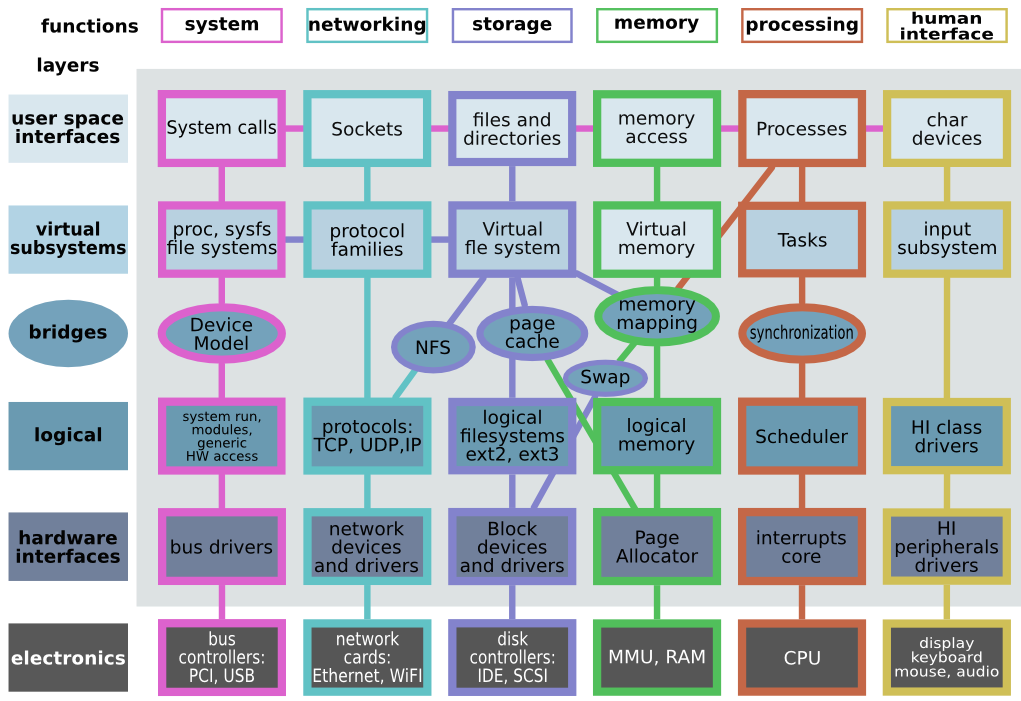
\includegraphics[width=1\textwidth]{KernelLinuxArchitectureImage}
    \caption{L'architettura del kernel Linux.}
     \label{fig:KernelLinuxArchitectureImage}
\end{figure}

Sebbene oggi il kernel possa essere compilato in modo da ottenere un'immagine binaria ridotta al minimo, e i driver possono essere caricati da moduli esterni, l'architettura originaria � chiaramente visibile: tutti i driver, infatti, devono avere una parte eseguita in kernel mode, anche quelli per cui ci� non sarebbe affatto necessario ( come ad esempio i driver dei file system ). 
\\
Attualmente il kernel Linux � distribuito con licenza GNU General Public License ed � in continua evoluzione grazie ad una vastissima comunit� di sviluppatori da ogni parte del mondo che contribuisce attivamente al suo sviluppo. 
\\
Il kernel Linux trova larghissima diffusione ed utilizzo: infatti grazie alla sua flessibilit� viene utilizzato dai personal computer ai grandi centri di calcolo, dai pi� moderni sistemi embedded agli smartphone.
\\
Android, il sistema mobile pi� diffuso al mondo, si basa su una versione lightweight del kernel Linux.

\end{section}
\begin{section}{Linux kernel v4.0}
Il 12 Aprile 2015 � stato rilasciata la versione 4.0 del kernel Linux. Il cambio di versione da 3.x a 4.0 non � dovuto a nessun particolare miglioramento del kernel: la nuova versione stabile sarebbe dovuta essere la 3.20 ma su proposta di Linus Torvalds si � deciso di incrementare la numerazione alla versione 4.0 per non creare confusione con numeri molto grandi. 
\\
La nuova versione del kernel, quindi, non introduce particolari nuove feature \cite{KernelLinuxChangelog}. Una delle novit� degna di nota � pero il \emph{live patching}: ovvero la possibilit� di installare pacchetti e estensioni al kernel senza dover riavviare la macchina. Questo pu� essere cruciale, ad esempio, per aspetti legati alla sicurezza.
\end{section}
\begin{section}{Linux networking}
I moduli del networking ( e relativi device driver ) occupano buona parte del codice del kernel Linux.
\\
Vi sono due strutture particolarmente importanti utilizzante largamente in tutto lo stack di rete del kernel Linux.
\begin{paragraph}{Socket buffer}
La struttura sk\_buff \cite{SocketBufferLinuxFoundation} mantiene le informazioni relative a ciascun pacchetto inviato o ricevuto lungo lo stack di rete di Linux.
\\
La struttura socket buffer contiene diversi campi che memorizzano le informazioni del pacchetto come il puntatore alla queue a cui � accodato o il socket a cui � associato.
\\
Essendo lo stack di rete implementato su pi� livelli, dove ciascun layer aggiunge ( o rimuove ) delle proprie informazioni di intestazione ad un messaggio, mantenere per ogni livello di rete una struttura diversa per identificare un certo pacchetto appartenente a quel dato layer potrebbe risultare parecchio oneroso in termini di memoria in quanto si finirebbe per copiare grandi quantit� di dati da un buffer ad un altro. Anche questo motivo, nel kernel Linux, si � deciso di mantenere un'unica struttura accessibile da qualsiasi layer dello stack di rete. 
\\
La struttura sk\_buff mantiene un union field per ciascun livello di rete dello stack TCP/IP ( trasporto, network, data-link ) dove ciascun campo ( h, nh, mac ) rappresenta un header di un protocollo di comunicazione adotabbile per quel livello. Ciascun campo di queste union punteranno poi effettivamente a un header per quel livello.
\\
Il campo \emph{data} punta all'inizio di tutti i dati relativi al pacchetto ( header compresi ) variando a seconda del layer in cui il socket buffer � utilizzato: in particolare quando una funzione ad un certo livello dello stack di rete tratta una struttura sk\_buff il campo data punter� all'header del messaggio per quel livello. Ad esempio in fase di ricezione di un pacchetto a livello network il campo nh di sk\_buff sar� inizializzato all'header puntato dal campo data. Se si vorr� accedere, per qualche motivo al payload del datagram IP si potr� farlo calcolando l'offset a partire dal puntatore data; inoltrando il pacchetto ad un layer superiore l'header relativo al livello di rete corrente potr� essere rimosso tramite la routine \textbf{skb\_pull()}. 
\\
In fase di invio il procedimento � molto simile ma con la difficolt� di dover appendere eventuali header man mano che si percorre lo stack di rete verso il basso. A tale scopo vi � una funzione di manipolazione delle strutture sk\_buff chiamata \textbf{skb\_reserve}, in genere invocata dopo un allocazione di un socket buffer, che consente di riservare dello spazio per gli header dei diversi protocolli.
\end{paragraph}

\begin{figure}[h]
    \centering
    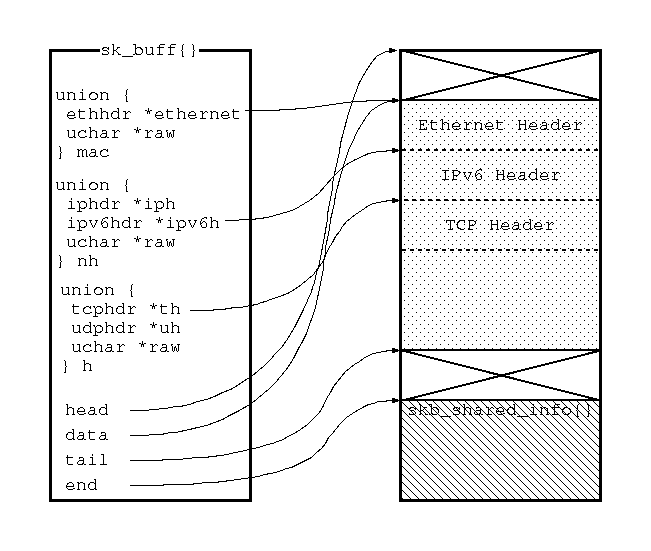
\includegraphics[width=1\textwidth]{SocketBufferImage}
    \caption{La struttura \emph{sk\_buff}.}
     \label{fig:SocketBufferImage}
\end{figure}

\begin{paragraph}{struct net\_device} questa struttura rappresenta una scheda di rete, anche virtuale: pu� essere infatti che ci si riferisca ad una scheda di rete virtuale ottenuta dopo aver effettuato un \emph{bonding}, ovvero � possibile assegnare un unico indirizzo IP a due o pi� NIC ( vedendole cos� come un unico device ) in modo da migliorare le performance. 
\\
La struttura net\_device contiene campi che identificano l'interfaccia di rete come il valore massimo della sua MTU e l'indirizzo MAC.
\\
Questa struttura viene inizializzata da un device driver non appena questo comincia la sua esecuzione.
\\
Le operazioni offerte verso il kernel dalla struttura net\_device sono contenute nel campo della struttura \textbf{const struct net\_device\_ops *netdev\_ops}; la struttura net\_device\_ops descrive un'interfaccia generica e omogenea per la gestione di tutti i device di rete.
\\
I campi contenuti nell'interfaccia net\_device\_ops non sono altro che semplici puntatori a funzione.
\\
Il device driver, in fase di inizializzazione, si occuper� di settare i campi della struttura net\_device\_ops mappando l'interfaccia offerta verso l'esterno con le funzioni implementate dal device driver per l'hardware specifico.
\end{paragraph}

Nello sviluppo del progetto di tesi � stato esteso il comportamento del workflow del kernel Linux per quanto riguarda la trasmissione di un datagram UDP. Per tanto, qui di seguito, descriveremo brevemente buona parte dei moduli che rendono possibile la trasmissione di un pacchetto UDP a partire da un applicazione fino al device driver.
\\
\begin{subsection}{Dall'app al device driver}
Quando viene invocata una routine che interagisce con la rete tramite socket  ( come ad esempio send, sendto o sendmsg ) il controllo viene passato al \emph{socket interface layer}: se il socket � di tipo TCP il controllo verr� dato alla funzione tcp\_sendmsg altrimenti, se di tipo UDP, alla primitiva udp\_sendmsg.
\\
Appena il flusso dell'esecuzione � passato alla routine udp\_sendmsg vengono effettuati alcuni controlli sui parametri passati come ad esempio sulla lunghezza specificata per il payload del datagram UDP o sugli indirizzi mittente e destinatario e le porte. Dopodich�, a seconda se specificato il flag UDP\_CORK o meno ( che consente quando abilitato tramite la system call \emph{setsockopt} di accumulare tutti i dati in output sul socket e inviarli in unico datagram quando disabilitato ), il controllo dell'esecuzione passer� alla primitiva di livello rete ip\_append\_data() oppure a ip\_skb\_make() che in entrambi casi, comunque, si appoggeranno sulla funzione \_\_ip\_append\_data() che tra le altre cose si occuper� di bufferizzare tutte le richieste di tramissione e di generare uno o pi� sk\_buff rappresentanti ciascun pacchetto ( o frammento ) IP. 
\\
A questo punto il flusso esecutivo torna a livello trasporto dove a un certo punto verr� invocata la primitiva udp\_push\_pending\_frames che genera l'header UDP e passa definitivamente il controllo a livello rete invocando la funzione ip\_push\_pending\_frame(). 
\\
In ip\_push\_pending\_frame() verr� generato l'header IP per ogni socket buffer in coda sul buffer in uscita per quel socket e dopo diversi controlli se il datagram IP necessita di frammentazione la funzione ip\_fragment si occuper� di frammentare il pacchetto IP in diverse strutture di tipo sk\_buff. 
\\
Tra i compiti a carico del livello network dello stack di rete vi � quello del \emph{routing}: in particolare a supporto del routing a livello rete vi � la funzione ip\_route\_output\_flow. 
\\
Se la fase di routing termina con successo verr� invocata la funzione di livello \emph{data-link} dev\_queue\_xmit() che, se l'interfaccia richiesta per la trasmissione � attiva, accoder� il socket buffer nella coda in uscita del net\_ device associato all' sk\_buff in invio e invocher� la funzione dev\_hard\_start\_xmit per cominciare a processare l'invio di un sk\_buff. 
\\
La funzione dev\_hard\_start\_xmit utilizzer� l'interfaccia esposta dalla struttura net\_device\_ops per cominciare la trasmissione in particolare invocher� la funzione ndo\_start\_xmit.
\\
Nel caso di un interfaccia di rete \emph{softMAC}, ovvero che il MLME ( MAC Sublayer Management Entity, ovvero dove viene implementata la logica del Medium Access Control ) � implementato via software ( vi sono dispositivi detti \emph{fullMAC} che implementano il MLME direttamente in hardware ) questa funzione si appogger� sul sottosistema mac80211.

\begin{paragraph}{Sottosistema mac80211}Il sottosistema mac80211 � stato rilasciato nel 2005 e si occupa di implementare la logica MLME per device softMAC interpretando e generando frame IEEE 802.11. Prima della sua adozione all'interno del kernel Linux la gestione e l'implementazione di IEEE 802.11 era lasciata ai device driver.
\\
Oggi la maggior parte dei device supportano questo sistema e in molti dei vecchi dispositivi i device driver sono stati riscritti tenendo conto di esso.
\\
Un device driver in fase di inizializzazione delle strutture net\_device da lui gestite pu� \emph{registrarle} presso il modulo mac80211.
\\
In questo modo alcuni dei campi contenuti nella struttura net\_device\_ops contenuti possono essere settati con dei callback offerti dal modulo mac80211.
\\
Alcuni campi della struttura net\_device\_ops debbono essere settati obbligatoriamente con i callback del modulo mac80211 nel caso si voglia beneficiare del sottosistema; altri sono opzionali  ( o pi� legati all'hardware specifico ) e possono essere implementati dal device driver stesso.
\\
In fase di trasmissione di un messaggio il controllo dal livello data-link viene ceduto, quindi, al sottosistema mac80211; questo � possibile in quanto, in fase di registrazione del device, la funzione ndo\_start\_xmit di net\_device\_ops viene mappata nella funzione del sottosistema mac80211 ieee80211\_monitor\_start\_xmit.
\\
Verr� poi invocata la entry point \textbf{ieee80211\_xmit} del modulo mac80211 che tra le altre cose si occupa dell'inizializzazione del frame 802.11 e del suo header. Per far ci� il sottosistema mac80211 si serve di una serie di handler appositamente settati, tra cui: 
\begin{itemize}
\item \textbf{ieee80211\_tx\_h\_dynamic\_ps} per la gestione del power saving.
\item \textbf{ieee80211\_tx\_h\_select\_key} si occupa di selezionare una chiave di cifratura. 
\item \textbf{ieee80211\_tx\_h\_michael\_mic\_add} si occupa di aggiungere il Message Integrity Code al frame IEEE 802.11.
\item \textbf{ieee80211\_tx\_h\_rate\_ctrl} che seleziona il bit rate con la quale il frame IEEE 802.11 deve essere trasmesso.
\item \textbf{ieee80211\_tx\_h\_sequence} calcola il \emph{sequence number} del frame e lo assegna all'header 802.11.
\item \textbf{ieee80211\_tx\_h\_fragment} si occupa, eventualmente, di frammentare il frame IEEE 802.11 in base al valore della MTU della scheda di rete wireless e a quella dell'access point.
\item \textbf{ieee80211\_tx\_h\_encrypt} cifra il frame IEEE 802.11 con l'algoritmo designato.
\item \textbf{ieee80211\_tx\_h\_calculate\_duration} si occupa di calcolare il campo \emph{duration} del frame IEEE 802.11 che indica per quanto tempo il canale sar� impegnato dalla trasmissione del frame.
\item \textbf{ieee80211\_tx\_h\_stats} setta una serie di variabili utili al mantenimento di alcune statistiche di trasmissione.
\end{itemize}
Una volta che il frame IEEE 802.11 � stato trasmesso la struttura socket buffer associata non viene immediatamente deallocata: mac80211 provveder� a ritrasmettere il messaggio per un certo numero di volte, dipendente dalla NIC e dallo stato in cui si trova la rete alla quale � connessa, qualora non dovesse ricevere l'ACK relativo a quel frame.
\\
Alla fine di questo processo viene invocata la routine ieee80211\_tx\_status che fornisce alcune informazioni riguardanti l'esito della trasmissione per un certo pacchetto come ad esempio quante volte il pacchetto � stato ritrasmesso e se � stato effettivamente consegnato o meno all'access point.
\\
A questo punto, sia che il frame IEEE 802.11 sia stato ricevuto dal first-hop o meno, il socket buffer associato viene definitivamente deallocato.
\end{paragraph}
\end{subsection}
\end{section}	

\begin{section}{Customizzazione kernel Linux}
Pu� esserci l'esigenza di personalizzare il proprio kernel per adattarlo alle proprie esigenze. Alcuni vantaggi che si possono ottenere dalla customizzazione del kernel sono:
\begin{itemize}
 \item Velocizzare l'avvio del sistema.
 \item Sfruttare un'ottimizzazione basata sul proprio processore per avere un sistema operativo un po' pi� reattivo.
 \item Ottenere una configurazione leggermente diversa e pi� adatta alla propria macchina.
 \item Cercare di migliorare le prestazioni del proprio dispositivo.
 \item Ridurre i consumi.
 \item Installare solo i moduli necessari.
 \item Rendere il sistema pi� leggero.
\end{itemize}
Per personalizzare il kernel, per�, serve una buona conoscenza della propria macchina, ed in particolare del proprio hardware.
Se non ci conosce il proprio hardware, infatti, si rischia di peggiorare le prestazione e si rischia di togliere dei moduli che possono influire sul funzionamento del sistema.

Non � necessario compilare un kernel nei casi in cui l'hardware non funzioni alla perfezione o le periferiche non vengano completamente riconosciute.
A volte per far riconoscere correttamente al sistema una data periferica basta caricare i moduli necessari con le dovute opzioni.
� utile ricompilare il kernel solo se tali moduli non sono presenti o se si � certi che i driver della periferica sono presenti solo in una versione diversa da quella attualmente in uso.
Inoltre, l'aumento di prestazioni tende a essere irrilevante, soprattutto su computer gi� veloci. 
� anche bene tenere presente che compilare un nuovo kernel significa, nella sostanza, cambiare sistema operativo, in quanto esso ne costituisce il motore; inoltre � richiesta un buona conoscenza del proprio hardware. 
%http://wiki.ubuntu-it.org/AmministrazioneSistema/CompilazioneKernel
% BIBLIOGRAFIA
\\
Dopo aver analizzato i vantaggi e gli svantaggi della personalizzazione del kernel, spieghiamo ora come si pu� fare la customizzazione.
Per modificare il kernel bisogna determinare quali driver sono necessari, compilare i kernel ed i moduli ed infine installare l'immagine del kernel.
\\
I passi da eseguire per portare a termine una customizzazione sono:
\begin{paragraph}{Scaricare una versione stabile del kernel ed estrarlo}
\begin{mdframed}[backgroundcolor=gray!30, topline=false,rightline=false,  leftline=false, bottomline=false ]
 \texttt{\# cd /directory/}
 \\
 \texttt{\# wget https://www.kernel.org/pub/linux/kernel/
 \\	v4.x/linux-4.0.1.tar.xz}
 \\
 \texttt{\# tar -xvJf linux-4.0.1.tar.xz}
 
\end{mdframed}
Il link indicato � quello relativo alla pagina ufficiale, dove si possono trovare le ultime versioni dei kernel. La versione scelta da noi � stata la 4.0.1 in quanto era l'ultima stabile.
\end{paragraph}
\begin{paragraph}{Scegliere la configurazione}
\begin{mdframed}[backgroundcolor=gray!30, topline=false,rightline=false,  leftline=false, bottomline=false ]
 
 \texttt{\# cd linux-4.0.1}
 \\
 \texttt{\# sudo apt-get install libncurses5}
 \\
 \texttt{\# sudo apt-get install libncurses5-dev}
 \\
 \\
 \texttt{\# sudo make menuconfig}
 
\end{mdframed}
Per poter eseguire il comando di menuconfig � necessario installare prima i componenti \emph{libncurses5}.
Una volta eseguito il comando di configurazione, si aprir� una finestra come quella indicata in figura ~\ref{fig:KernelLinuxMenuconfig}
Nel caso in cui si volessero aggiungere o rimuovere moduli, bisogner� andare a selezionarli all'interno di questo menu.

\begin{figure}[h]
    \centering
    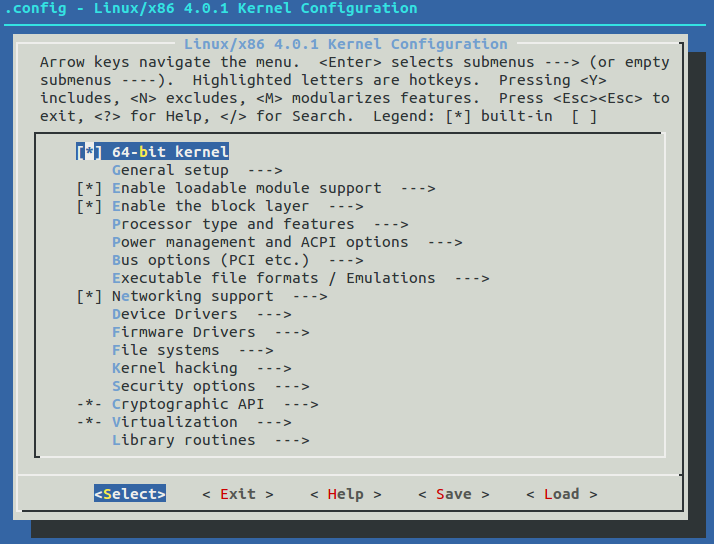
\includegraphics[width=1\textwidth]{KernelLinuxMenuconfig}
    \caption{Esecuzione del comando menuconfig.}
     \label{fig:KernelLinuxMenuconfig}
\end{figure}
\end{paragraph}

\begin{paragraph}{Compilare il Kernel}
\begin{mdframed}[backgroundcolor=gray!30, topline=false,rightline=false,  leftline=false, bottomline=false ]
 \texttt{\# sudo make } 
\end{mdframed}
Con questo comando si va a compilare il kernel. Questa operazione pu� richiedere diverso tempo, in particolare in dispositivi con prestazione ridotte.
� possibile anche specificare l'opzione -jN con N che indica il numero di core pi� uno ( ad esempio \emph{-j5} per un quad-core ) per velocizzare l'operazione.

\end{paragraph}

\begin{paragraph}{Compilare i moduli ed installarli}
\begin{mdframed}[backgroundcolor=gray!30, topline=false,rightline=false,  leftline=false, bottomline=false ]
 \texttt{\# sudo make modules} 
 \\
 \texttt{\# sudo make modules\_install} 
\end{mdframed}

\end{paragraph}


\begin{paragraph}{Installare il Kernel}
\begin{mdframed}[backgroundcolor=gray!30, topline=false,rightline=false,  leftline=false, bottomline=false ]
 \texttt{\# sudo make install} 
 \\
 \texttt{\# sudo reboot} 
 
\end{mdframed}
Come ultima operazione si va ad installare l'immagine del nuovo kernel.
Una volta riavviato il sistema � possibile utilizzare il proprio kernel customizzato.
\end{paragraph}




\end{section}

\end{chapter}
%\end{document}


%\documentclass[12pt,a4paper,openright,twoside]{book}
%\usepackage[italian]{babel}
%\usepackage[latin1]{inputenc}
%\usepackage{fancyhdr}
%\usepackage{indentfirst}
%\usepackage{graphicx}
%\graphicspath{ {Images/}  }
%\usepackage{newlfont}
%\usepackage{amssymb}
%\usepackage{amsmath}
%\usepackage{latexsym}
%\usepackage{amsthm}
%
%
%\pagestyle{fancy}\addtolength{\headwidth}{20pt}
%\renewcommand{\chaptermark}[1]{\markboth{\thechapter.\ #1}{}}
%\renewcommand{\sectionmark}[1]{\markright{\thesection \ #1}{}}
%\rhead[\fancyplain{}{\bfseries\leftmark}]{\fancyplain{}{\bfseries\thepage}}
%\cfoot{}
%
%\linespread{1.3}    
%
%\begin{document}
\begin{chapter}{Lo stack di rete}
In questo capitolo si vuole presentare la suite di protocolli utilizzata nel progetto di tesi.
\\
Verr� descritto brevemente il modello ISO/OSI per poi soffermarsi con particolare attenzione sulla tecnologia Wi-Fi e sui protocolli toccati dal progetto di tesi.
\\
ISO/OSI � uno standard che definisce un modello composto su pi� livelli: ogni \emph{layer} si occupa di uno specifico aspetto delle comunicazioni di rete fornendo delle funzionalit� a livello superiore e sfruttando le astrazioni fornite dal livello immediatamente inferiore.
\\
In questo modo � possibile ridurre la complessit� non banale delle comunicazioni di rete. 

%ISO/OSI and TCP/IP
\begin{section}{Il modello ISO/OSI}
Il modello OSI (Open System Interconnection)\cite{ISOOSIBibliography} � uno standard per le reti di calcolatori stabilito da ISO (International Standard Organization) che definisce l'architettura logica di rete come una struttura a strati composta da una pila di protocolli di comunicazione di rete suddivisa in 7 livelli, i quali insieme espletano in maniera logico-gerarchica tutte le funzionalit� della rete.
\\
Ciascun layer racchiude in s�, a livello logico, uno o pi� aspetti fra loro correlati della comunicazione fra due nodi di una rete. 
\\
I layers vanno dal livello fisico (quello del mezzo trasmissivo, ossia del cavo twisted pair o delle onde radio) fino al livello delle applicazioni, attraverso cui si realizza la comunicazione di alto livello. Come gi� accennato ciascun livello fornisce servizi e funzionalit� al livello superiore utilizzando le astrazioni fornite dal livello inferiore. Ma vediamo brevemente le funzioni di ciascun livello all'interno dello stack ISO/OSI.
\\
%Physical Layer
\begin{paragraph}{Physical layer}
Si occupa di trasmettere dati non strutturati attraverso un mezzo fisico e di controllare la rete, gli hardware che la compongono e i dispositivi che permettono la connessione.
In questo livello vengono decisi diversi aspetti legati al mezzo fisico come ad esempio le tensioni scelte per rappresentare i valori logici dei bit trasmessi, la durata in microsecondi del segnale che identifica un bit, la modulazione e la codifica utilizzata e l'eventuale trasmissione simultanea in due direzioni ( full-duplex ).
\end{paragraph}
%Datalink layer
\begin{paragraph}{Data link layer}
Questo livello si occupa in primis di formare i dati da inviare attraverso il livello fisico, incapsulando il pacchetto proveniente dallo strato superiore in un nuovo pacchetto provvisto di un nuovo header ( intestazione ) e tail ( coda ). Questa frammentazione dei dati in specifici pacchetti � detta \emph{framing} e i singoli pacchetti sono chiamati \emph{frame}.
\\
Il livello data link effettua, inoltre, un controllo degli errori e delle perdite di segnale in modo tale da far apparire, al livello superiore, il mezzo fisico come una linea di trasmissione esente da errori di trasmissione.
\end{paragraph}
%Network layer
\begin{paragraph}{Network layer}
Si occupa di rendere i livelli superiori indipendenti dai meccanismi e dalle tecnologie di trasmissione usate per la connessione. Si prende carico della consegna a destinazione dei pacchetti.
� responsabile del \emph{routing} ovvero della scelta ottimale del percorso di rete da utilizzare per garantire la consegna delle informazioni dal mittente al destinatario, scelta svolta dal router attraverso dei particolari algoritmi di routing e tabelle di routing.
\\
� responsabile, inoltre, della conversione dei dati nel passaggio fra una rete ed un'altra con diverse caratteristiche, come ad esempio reti che adottano diversi protocolli di rete: si deve occupare quindi di tradurre gli indirizzi di rete, valutare la necessit� di frammentare i pacchetti dati se la nuova rete ha una diversa Maximum Transmission Unit (MTU) e di valutare la necessit� di gestire diversi protocolli attraverso l'impiego di gateway. L'unit� dati fondamentale � il pacchetto o \emph{datagram}.
\end{paragraph}
%Transport layer
\begin{paragraph}{Transport layer}
Permettere un trasferimento di dati trasparente e affidabile (implementando anche un controllo degli errori e delle perdite) tra due host. 
\\
� il primo livello realmente \emph{end-to-end}, cio� da host sorgente a destinatario. Si occupa di stabilire, mantenere e terminare una connessione, garantendo il corretto e ottimale funzionamento della sottorete di comunicazione nonch� del controllo della congestione: si occupa, cio�, di evitare che troppi pacchetti dati arrivino allo stesso router contemporaneamente causando cos� una perdita dei pacchetti stessi.
\\
A differenza dei livelli precedenti, che si occupano di connessioni tra nodi contigui di una rete, il transport layer si occupa solo del punto di partenza e di quello finale.
Si occupa anche di effettuare la frammentazione dei dati provenienti dal livello superiore in pacchetti, detti generalmente \emph{segmenti} nel caso di connessione TCP o datagram nel caso di trasmissione UDPlayer, e trasmetterli in modo efficiente ed affidabile usando il livello rete ed isolando da questo i livelli superiori. Inoltre, si preoccupa di ottimizzare l'uso delle risorse di rete e di prevenire la congestione.
\end{paragraph}
%Session layer
\begin{paragraph}{Session layer}
Consente di aggiungere, ai servizi forniti dal livello di trasporto, servizi pi� avanzati, quali la gestione del dialogo ( mono o bidirezionale ), la gestione del token (per effettuare mutua esclusione) o la sincronizzazione ( inserendo dei checkpoint in modo da ridurre la quantit� di dati da ritrasmettere in caso di gravi malfunzionamenti ).
Si occupa anche di inserire dei punti di controllo nel flusso dati: in caso di errori nell'invio dei pacchetti, la comunicazione riprende dall'ultimo punto di controllo andato a buon fine.
\end{paragraph}
%Presentation layer
\begin{paragraph}{Presentation layer}
Si occupa di trasformare i dati forniti dalle applicazioni in un formato standard e di offrire servizi di comunicazione comuni, come la crittografia, la compressione del testo e la ri-layerformattazione.
\end{paragraph}
%Application layer
\begin{paragraph}{Application layer}
Il livello Applicazione � quello pi� vicino al livello utente. Fornisce un'interfaccia tra le applicazioni e lo stack di rete sottostante che si occupa dell'invio di messaggi. I protocolli di livello applicazione si occupano, quindi, dello scambio di informazioni tra apps in esecuzione sull'host sorgente e quello destinatario della comunicazione.
\end{paragraph}
\end{section}
%ISO/OSI vs TCP/IP
\begin{section}{ISO/OSI vs TCP/IP}
TCP/IP, sviluppato inizialmente dal dipartimento della difesa americano e utilizzato nei primi computer UNIX-based, attualmente � lo \emph{standard de facto} per tutte le comunicazioni internet. 
\\
TCP/IP, come l'OSI model, � strutturato su pi� livelli, alcuni dei quali molto simili per caratteristiche e funzionalit� a quelli di ISO/OSI: TCP/IP accorpa in un unico layer funzionalit� contenute su pi� livelli del modello OSI. 
\\
\\
TCP/IP � l'approccio utilizzato in ogni tipo di comunicazione internet. L'obbiettivo di ISO/OSI invece � quello fornire uno standard da usare come guideline per la definizione di protocolli e applicazioni internet.
\\
\\
I layer nello stack TCP/IP sono quattro e sono cos� organizzati rispetto al modello OSI come illustrato nella figura \ref{fig:ISOOSI}.
\\
\\
\begin{figure}[h]
    \centering
    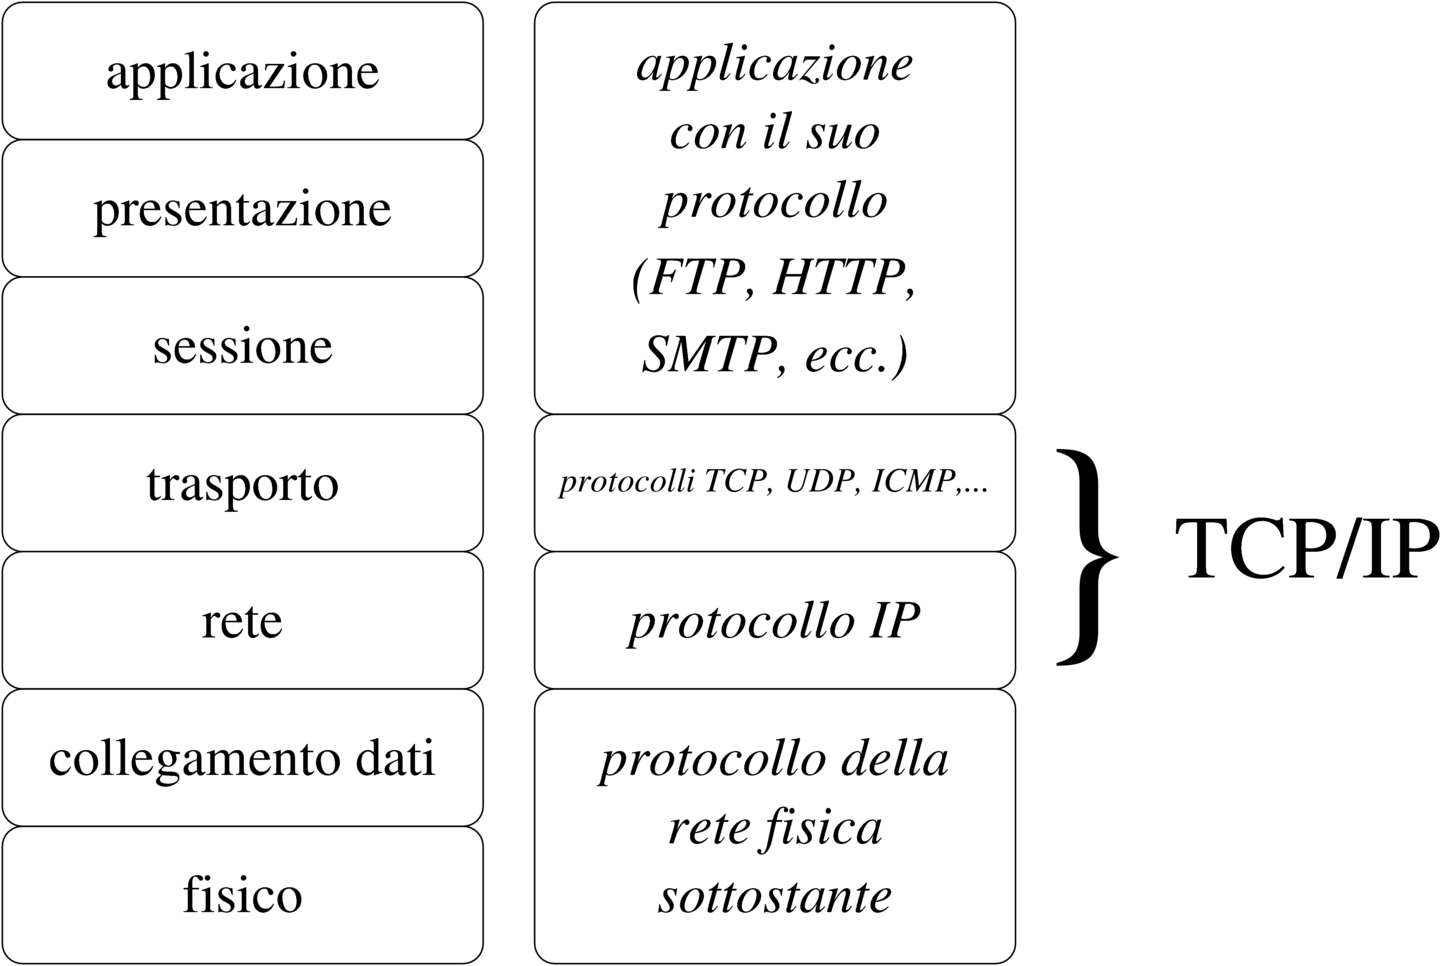
\includegraphics[width=1\textwidth]{ISOOSI}
    \caption{Stack di rete ISO/OSI e TCP/IP}
     \label{fig:ISOOSI}
\end{figure}
 
\end{section}

\begin{section}{Wi-Fi}
Wi-Fi indica una tecnologia che consente a calcolatori collocati su di una stessa WLAN ( Wireless Local Area Network ) di comunicare senza fili attraverso specifiche frequenze di onde radio secondo le specifiche dello standard \textbf{IEEE 802.11}. Sempre pi� dispositivi dispongono di interfacce di rete Wi-Fi: dai laptop, agli smartphone fino agli elettrodomestici di ultima generazione, che possono essere cos� interconnessi entro un certo raggio di copertura.
\\
La tecnologia Wi-Fi pu� essere usata per fornire connettivit� internet ai dispositivi presenti nel raggio di copertura della WLAN se la Local Area Network � connessa ad internet. % menzionare ISP ???????!!! BOOOOHHH
\\
\begin{subsection}{WLAN architecture and types}
L'architettura di una WLAN � caratterizzata da diverse componenti.
\begin{paragraph}{Stazioni}
In una WLAN ciascun dispositivo munito di Wireless Network Interface Controllers (WNICs), e che quindi pu� comunicare senza fili, � detto stazione.
Vi sono due categorie di stazioni:
\begin{itemize}
\item \textbf{Access points (AP)} ovvero dispositivi elettronici che ricevono/trasmettono segnali radio da/verso nodi mobili equipaggiati con schede di rete Wi-Fi.
\item \textbf{Clients}, tutti i nodi mobili che possono essere equipaggiati con una wireless network interface come ad esempio laptops, smartphones o workstations.
\end{itemize}
\end{paragraph}

\begin{paragraph}{Basic service set}
Il Basic Service Set (BSS) � un insieme di tutte le stazioni che possono comunicare tra loro. Ciascun BSS ha un proprio identificativo detto BSSID che corrisponde al indirizzo MAC dell'access point che serve i diversi clients per quella BSS.
\\
Vi sono due tipi di BSS:
\begin{itemize}
\item Indipendent BSS (IBSS) ovvero una \emph{rete ad-hoc} caratterizzata dall'assenza di un access point. Questo tipo di BSS non pu� quindi essere interconnesso con altri Basic Service Set.
\item Infrastructure BSS caratterizzati dalla presenza di un access point, un BSS di questo tipo pu� essere connesso con altri Basic Service Set.
\end{itemize}
\end{paragraph}


%EES
\begin{paragraph}{Extended Service Set}
Un Extended Service Set (ESS) � un insieme di BSS interconnessi tra loro. Gli access points in un ESS sono connessi tra loro da un \emph{Distribution System}. Ciascun EES � caratterizzato da una stringa identificativa lunga al massimo 32 byte detta SSID. 
\end{paragraph}

%Distribution System
\begin{paragraph}{Distribution System}
Il Distribution System (DS) inter-connette tra loro gli access point di diversi EES. Un access point pu� essere principale, di inoltro o remoto. Un access point principale � collegato tipicamente alla rete cablata. Un access point di inoltro trasmette i dati fra le stazioni remote e principali. Un access point remoto accetta i collegamenti dai client senza fili e li passa a quelli di inoltro o quelli principali. 
\end{paragraph}
\\ 
\\	%WLAN types
Esistono due tipologie di rete WLAN che differiscono dalle modalit� di comunicazione:
\begin{itemize}
\item Infrastructure, i nodi comunicano tra loro attraverso a una base station che funge da wireless access point.
\item Reti ad-hoc, ovvero una rete dove le stazioni possono comunicare peer-to-peer (P2P) senza alcun access point. Questo viene realizzato tramite IBSS.
\end{itemize}

\end{subsection}
\end{section}

%IEEE 802.11
\begin{section}{IEEE 802.11}
IEEE 802.11 � uno standard di trasmissione per reti WLAN, operanti su frequenze 2.4 e 5 GHz, che definisce un'interfaccia di comunicazione base per trasmissioni Wi-Fi. Le specifiche definite nello standard 802.11 si focalizzano sul livello fisico e MAC del modello ISO/OSI. 
Il sistema di numerazione 802.11 � dovuto ad IEEE che utilizza 802.x per indicare una famiglia di standard per le comunicazione di rete tra cui lo standard \emph{Ethernet} (IEEE 802.3). Per tanto IEEE 802.11 si adegua perfettamente agli altri standard 802.x per reti locali wired e le applicazioni che lo utilizzano non dovrebbero notare nessuna differenza logica, una degradazione delle performance, invece, � tuttavia possibile.
IEEE 802.11b  � stato il primo protocollo largamente utilizzato seguito da 802.11a, 802.11g, 802.11n, e 802.11ac. Vi sono altri standard nella famiglia 802.11 (c-f, h, j) che sono per lo pi� piccole modifiche, estensioni o correzioni alle precedenti specifiche.
\\
Per quanto concerne le performance, lo stream data rate pu� arrivare fino a 780 Mbit/s in 802.11ac grazie anche alla tecnologia MIMO (Multiple-Input and Multiple-Output) che consente di aumentare la capacit� del canale trasmissivo usando pi� trasmittenti e ricevitori, sfruttando cos� il fenomeno del \emph{multipath-propagation}, ovvero un segnale radio pu� raggiungere un ricevitore attraverso diversi percorsi, \emph{path}.

%Physical Layer in 802.11
\begin{subsection}{Physical layer in 802.11}
Come gi� detto, IEEE 802.11\cite{IEEE802dot11Bibliography} utilizza le bande di frequenza  2.4 e 5 GHz e a \emph{livello fisico} vengono usate delle tecniche di modulazione \emph{half-duplex}: in particolare viene utilizza la Orthogonal Frequency-Division Multiplexing (OFDM) che utilizza un numero elevato di sotto-portanti ortogonali tra di loro, oppure quella chiamata Direct Sequence Spread Spectrum (DSSS), che � una tecnologia di trasmissione a banda larga nella quale ogni bit viene trasmesso come una sequenza ridondante di valori, detti chip, rendendola cos� pi� resistente ad eventuali interferenze.
\end{subsection}

%MAC Media Access Control
\begin{subsection}{Media Access Control}
Media Access Control (MAC)\cite{ISOOSIBibliography} � un \emph{sublayer} del livello \emph{data link} del modello OSI. MAC fornisce meccanismi di indirizzamento e di controllo di accesso al canale che consentono a nodi mobili di comunicare attraverso una rete con medium condiviso. L'hardware che implementa MAC � detto \emph{media access controller}.
Le funzioni principali del MAC sono quindi quelle di regolamentare l'accesso al mezzo fisico, frammentazione dati in frame e riconoscimento degli stessi frame e controllo degli errori.
\end{subsection}

%controllo dell'accesso
\begin{subsection}{CSMA/CA}
Carrier Sense Multiple Access with Collision Avoidance\cite{IEEE802dot11Bibliography}  � un protocollo di accesso multiplo in cui i nodi cercano di evitare a priori il verificarsi di collisioni in trasmissione. Questo approccio � l'ideale per tipologie di reti nella quale non risulta possibile ( oppure poco affidabile e dispendioso ) rilevare un'avvenuta collisione.
\\
Quando un nodo vuole effettuare una trasmissione ascolta il canale \emph{(listen-before-talk)} ( LBT ): se il canale risulta \emph{idle}, il nodo aspetta un certo \emph{DISF time ( Distribuited Inter Frame Space )} trascorso il quale, se il canale risulta ancora libero, comincer� a trasmettere. A termine della trasmissione il nodo sorgente aspetter� per un certo intervallo \emph{SISF ( Short Inter Frame Space )}, pi� piccolo di DISF, la ricezione di un \emph{ACK}. Se il nodo sorgente non riceve alcun ACK ritrasmetter� il messaggio per un certo numero di volte.
\\
Per tutta la durata della trasmissione, e per la durata dello SISF time, le altre stazioni, trovando il canale occupato, non avvieranno altre comunicazioni evitando cos� collisioni. La durata dello SISF, inferiore a quello dell'intervallo di DISF, assicura che nessuna stazione comincer� una trasmissione prima della ricezione dell'eventuale messaggio di acknowledgment da parte del nodo che ha appena concluso la trasmissione.
\\
Nel caso in cui una stazione volesse trasmettere, e rileva il canale occupato, attender� per un certo intervallo di tempo casuale, detto intervallo di \emph{back-off}, prima di riprovare a trasmettere. L'intervallo di back-off � realizzato per mezzo di un timer che decrementa il valore di un contatore, inizializzato con il valore dell'intervallo, solamente nei periodi di inattivit� del canale, ovvero quando non vi sono trasmissioni; il valore del contatore rester� invece invariato durante i periodi di trasmissione da parte di altre stazioni (\emph{frozen back-off}). Quando il valore del contatore raggiunger� lo zero la stazione effettuer� un nuovo tentativo di trasmissione. Questo meccanismo di accesso al mezzo � detto \emph{Basic Access Mechanism}
% devo scrivere come calcolare backoff time???????????!!!!! BOH
\end{subsection}
%Hide node problem
\begin{subsection}{Il problema dei nodi nascosti}
Il problema dei nodi nascosti in una rete wireless s� ha quando un nodo all'interno della rete � visibile da un Access Point ma non da tutte le altre stazioni collegate al medesimo AP. Questo pu� comportare una serie di problemi per quanto riguarda il controllo dell' accesso al mezzo.

\begin{figure}[h]
    \centering
    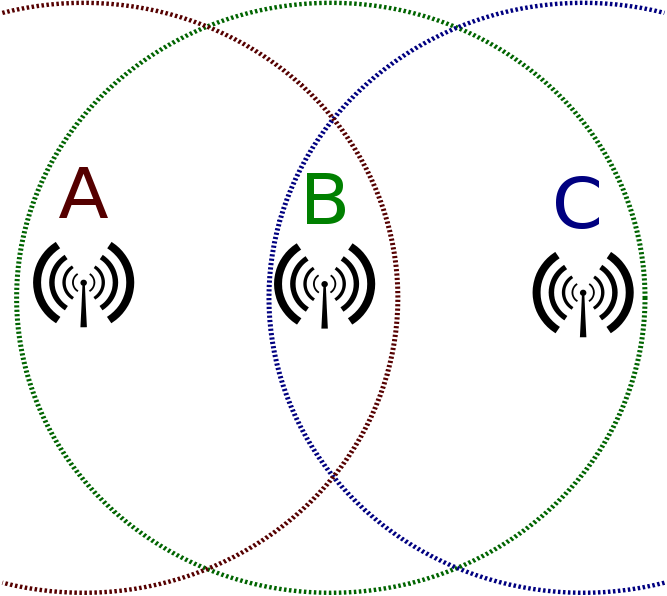
\includegraphics[width=0.3\textwidth]{HiddenNodeProblemImage}
    \caption{Il problema dei nodi nascosti}
     \label{fig:HiddenNodeProblemImage}
\end{figure}

Come si pu� vedere dalla figura \ref{fig:HiddenNodeProblemImage} la stazione A e la C sono nel raggio di copertura della stazione B. Per qualche motivo (come pu� essere la distanza o un ostacolo) A e C non possono comunicare direttamente e quindi non possono nemmeno rilevare (\emph{sensing}) la portante trasmessa dall'altra stazione verso la stazione centrale B. In particolare si possono quindi verificare delle collisioni quando sia A che C, rilevando il canale libero, effettuano in contemporanea una trasmissione verso B.
\\
Per ovviare a questo problema IEEE 802.11 definisce un meccanismo opzionale che introduce due tipi di pacchetti di controllo, in particolare:
\begin{itemize}
\item \emph{RTS} ( Request To Send ), quando un nodo vuole trasmettere, prima di inviare il frame vero e proprio, invia al destinatario un pacchetto di tipo RTS contenente destinatario del messaggio, mittente e durata della trasmissione che seguir�. 
\item \emph{CTS} ( Clear To Send ), quando un nodo riceve un pacchetto di tipo RTS risponde con un pacchetto di tipo CTS contenente, essenzialmente, le stesse informazioni contenute nel frame di tipo RTS; quando il nodo mittente avr� ricevuto il frame CTS potr� cominciare l'inoltro del frame precedentemente annunciato tramite il rispettivo RTS.
\end{itemize}
I pacchetti RTS e CTS vengono inoltrati a tutte le stazioni comprese, quindi, anche quelle nascoste al mittente, che si metteranno in attesa per tutta la durata della trasmissione come specificato dai frame di controllo.
\\
Questo meccanismo non � del tutto esente da collisioni. Infatti, le collisioni possono ancora avvenire durante lo scambio dei pacchetti di controllo: ad esempio, due stazioni mandano contemporaneamente una Request To Send. Nonostante ci�, la probabilit� di collisione risulta essere pi� bassa e meno significativa rispetto all'approccio che non fa uso dei pacchetti RTS/CTS, in quanto i frame di controllo hanno una dimensione molto ridotta (fino a 2347 bytes).
\\
Se una stazione vuole trasmettere un pacchetto di dimensione inferiore al frame di controllo, il messaggio verr� inoltrato immediatamente senza prima generare il corrispettivo RTS.

\begin{figure}[h]
    \centering
    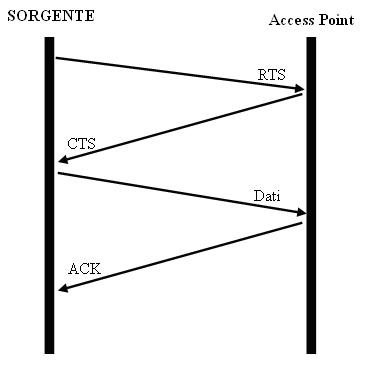
\includegraphics[width=0.7\textwidth]{HiddenNodeFourWayHandshake}
    \caption{\emph{Four-way handshake} via RTS/CTS}
     \label{fig:HiddenNodeFourWayHandshake}
\end{figure}

\end{subsection}
%IEEE 802.11 frames
\begin{subsection}{IEEE 802.11 frame}
IEEE 802.11 definisce tre tipologie di frame:
\begin{itemize}
\item	DATA, contengono meramente dati.
\item CTRL, servono per facilitare l'interscambio di data frame tra le stazioni; appartengono a questa categoria i frame RTS, CTS e ACK.
\item MGMT, frame utili al mantenimento della comunicazione; i \emph{beacon frame} ( frame inviato periodicamente da un AP per annunciare al sua presenza e il suo SSID ) appartengono a questa categoria.
\end{itemize}
Ciascun frame � composto da un \emph{MAC header}, un \emph{payload} e un \emph{frame check sequence ( FCS )}.

\begin{figure}[h]
    \centering
    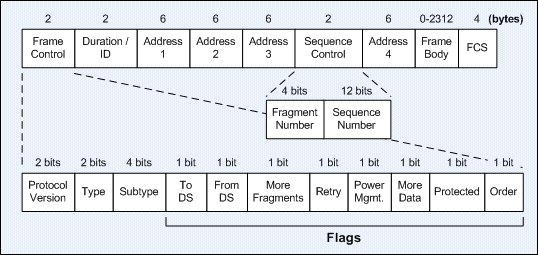
\includegraphics[width=\textwidth]{802dot11FrameImage}
    \caption{IEEE 802.11 frame}
     \label{fig:802dot11FrameImage}
\end{figure}

\begin{paragraph}{MAC header}
I primi due byte del MAC header contengono un campo molto interessante, il \emph{frame control}. Il frame control contiene diversi sotto-campi:
\begin{itemize}
\item Protocol Version, ovvero due bit rappresentanti la versione del protocollo, posto sempre a zero; altri valori sono riservati per un uso futuro.
\item Type, due bit identificanti appunto il tipo di frame.
\item Subtype, quattro bit che identificano il sottotipo del frame; ad esempio come beacon � un sottotipo di MGMT.
\item ToDS \& FromDS, ciascun campo occupa un bit e indica se un data frame � diretto o proviene da un distribution system. I frame di tipo CTRL e MGMT hanno entrambi i flag settati a zero.
\item More Fragments, bit settato quando un pacchetto viene frammentato in pi� frame per la trasmissione; tutti i pacchetti con eccezione dell'ultimo inviato avranno questo flag settato.
\item Retry, indica se un frame � stato oggetto di ritrasmissione; utile per eliminare eventuali frame duplicati.
\item Power Management: indica il \emph{power management state} (ovvero se la stazione � in power-save state o meno) del mittente, settato dopo la trasmissione. Gli AP non setteranno mai questo bit in quanto sempre attivi per la gestione delle connessioni.
\item More Data, questo bit indica che c'� almeno un pacchetto disponibile; settato dagli AP per facilitare le stazioni in power-save mode.
\item Protected, indica se il payload del frame � stato cifrato o meno.
\item Order, questo bit � settato solamente quando i frame sono inviati in ordine uno dietro l'altro; spesso ci� non avviene per motivi di performance.
\end{itemize}
Gli altri campi contenuti nell'header MAC sono la durata di trasmissione, gli indirizzi MAC ( \emph{source}, \emph{destination}, \emph{transmitter} e \emph{receiver} ) e il \emph{Sequence Control}.
\\
Il campo Sequence Control � composto da due byte usato per identificare l'ordine dei frame spediti. I primi 4 bit corrispondono al \emph{fregmentation number} e gli ultimi 12 bit sono il \emph{sequence number}. Il fragmentation number indica il numero di ogni pacchetto precedentemente frammentato, il sequence number, invece, � un valore modulo 4096 assegnato ad un frame e rimane costante per ogni ritrasmissione o per ciascun fragment di quel pacchetto.
\end{paragraph}
\begin{paragraph}{Payload}
Il Payload ha dimensione variabile da 0 a 2304 byte; contiene informazioni provenienti dai livelli di rete superiori. Le informazioni provenienti dai livelli superiori, prima di essere incapsulate in un frame MAC, sono incapsulate in un frame di tipo IEEE 802.2 che definisce LLC ( Logical Link Protocol ) che rappresenta il sublayer superiore del livello Data-Link del modello OSI. LLC offre un'interfaccia di comunicazione omogenea verso il livello data link al layer superiore ( a differenza di MAC che � dipendente dal mezzo trasmissivo utilizzato ). Il pacchetto 802.2 � detto PDU ( Protocol Data Unit ) e il suo header contiene informazioni di controllo aggiuntive e pu� essere esteso con SNAP ( Subnetwork Access Protocol ) che consente di specificare il tipo di protocollo ( \emph{Protocol ID} field ) a cui appartengono i dati contenuti nel payload della PDU. Questa estensione pu� essere molto utile ad esempio in fase di ricezione di un frame: � possibile vedere a quale protocollo appartengono i dati contenuti nel payload e consegnare, quindi, i dati al giusto protocollo dello stack di rete ( si basti pensare anche solamente ad IPv4 vs IPv6 ).
\end{paragraph}
\begin{paragraph}{Frame check sequence (FCS)}
Spesso detto anche \emph{Cyclic Redundancy Check} ( CRC ), permette di verificare l'integrit� di un frame appena ricevuto: quando un frame sta per essere spedito la stazione sorgente calcola questo valore e lo appende al frame IEEE 802.11. Quando un nodo riceve il frame ricalcola l'FCS sulla base dei dati ricevuti e lo confronta con il valore contenuto nel \emph{trailer} del pacchetto; se i due valori coincidono il frame non ha subito delle modifiche durante la trasmissione.
\\
Il campo FCS occupa gli ultimi quattro byte del frame IEEE 802.11 
\end{paragraph}
\end{subsection}
% IEEE 802.11 security. http://www.sans.org/reading-room/whitepapers/wireless/overview-80211-wireless-network-security-standards-mechanisms-1530
\begin{subsection}{Security in IEEE 802.11}
Data la sempre pi� larga diffusione delle reti Wi-Fi e dalla natura del loro segnale ( � molto difficile controllare quale dispositivo riceve il segnale radio ) la sicurezza � un aspetto molto importante e assolutamente da non sottovalutare in 802.11.
Nel corso degli anni sono stati sviluppati e proposti diversi approcci per rendere le reti WLAN sempre meno sensibili a intercettazioni e attacchi da parte di terzi.
%ACL
\begin{paragraph}{Access Control List}
Un primo banale approccio � quello dell'\emph{access control list}. L' Access Point mantiene una lista degli indirizzi MAC autorizzati alla comunicazione: l' AP riceve messaggi provenienti solo dai clients presenti nell'access control list. Qualsiasi messaggio proveniente da una stazione non presente nella lista sar� ignorato.
\\
Questo approccio presenta due grandi difetti. Innanzitutto fornisce solamente una politica di controllo degli accessi senza fornire nessun meccanismo di protezione sui dati trasmessi. Inoltre questo approccio pu� essere facilmente raggirato tramite una tecnica di \emph{MAC spoofing}. In particolare tramite un software di \emph{wireless network analysis} � possibile monitorare il traffico delle rete WLAN vicine e quindi captare informazioni sensibili da eventuali messaggi trasmessi in chiaro: data la mancanza di confidenzialit� nei messaggi trasmessi su reti che adottano esclusivamente la politica dell'Access Control List come protezione � possibile quindi risalire ad indirizzi MAC autorizzati alla comunicazione. A questo punto � possibile modificare l'indirizzo MAC dell'interfaccia di rete ( possibile sia in ambiente UNIX che Windows ) per impersonare un altro client della rete WLAN.
\end{paragraph}
%WEP
\begin{paragraph}{WEP ( Wired Equivalent Privacy )}
WEP ( Wired Equivalent Privacy )\cite{SecurityBibliography} � stato il primo protocollo di sicurezza definito nello standard IEEE 802.11. L'obbiettivo di WEP � quello di garantire confidenzialit� e integrit� del traffico trasmesso in maniera wireless. Il nome � dovuto al fatto che WEP � stato pensato per fornire confidenzialit� sui dati trasmessi paragonabile a quella delle reti cablate.
\\
WEP sfrutta il cifrario a chiave simmetrica RC4 con chiave a 64 o 128 bit. La chiave WEP utilizzata � la concatenazione di due valori: il primo dinamico detto Initialization Vector (IV) e la seconda parte statica corrispondente alla chiave segreta condivisa. Il vettore di inizializzazione � una sequenza di 24 bit generata casualmente al momento dell'invio del frame da parte dell'interfaccia di rete ( per ogni trasmissione verr� generato un IV in quanto RC4 � un \emph{cifrario a flusso} ). A seconda della lunghezza della WEP key la chiave segreta condivisa sar� quindi lunga 40 bit nel caso di una WEP key di 64 bit oppure 104 bit nel caso di una chiave a 128 bit. 
\\
Al momento dell'invio di un frame la stazione sorgente genera il vettore di inizializzazione e lo concatena alla shared key. Una volta che la WEP key � stata formata viene data in pasto all'algoritmo di cifratura RC4 per produrre una stringa pseudo-casuale della lunghezza pari ai dati da trasmettere. Una volta generata la stringa pseudo-random quest'ultima viene posta in XOR dalla scheda di rete con i dati da trasmettere: il risultato assieme al vettore di inizializzazione in chiaro sar� appeso a un header IEEE 802.11 e trasmesso verso il destinatario del messaggio.
\\
Quando il nodo destinatario riceve il messaggio cifrato come prima cosa legge l'IV lo concatena alla shared key e calcola la psudo-random string via RC4 ( data la stessa WEP key la stringa pseudo-casuale generata sar� sempre uguale ). Il risultato ottenuto viene posto in XOR con i dati cifrati contenuti nel frame ottenendo cos� il testo in chiaro. 
\\
A partire dal 2003 questo approccio non � pi� considerato sicuro a causa dalle numerose falle presenti in WEP e dalla facilit� con cui RC4 pu� essere violato.
\end{paragraph}
%WPA
\begin{paragraph}{WPA ( Wi-Fi Protected Access)}
Una volta scoperte le falle che affliggevano WEP � iniziato lo sviluppo del protocollo IEEE 802.11i, un nuovo standard considerato pienamente sicuro. Nel frattempo viene rilasciato dalla Wi-Fi Alliance WPA ( Wi-Fi Protected Access )\cite{SecurityBibliography} che soddisfa molte delle linee guide di IEEE 802.11i
Il WPA � caratterizzato da tre componenti principali:
\begin{itemize}
\item TKIP (Temporal Key Integrity Protocol), � la componente che pi� va a sostituire la logica di WEP risolvendo la maggior parte delle sue vulnerabilit�. Una delle innovazioni pi� importanti � quella che ogni messaggio trasmesso viene cifrato con una chiave diversa in modo tale da non esporre la chiave principale.
\\
Molte funzioni di crittografia sono built-in nell'hardware di rete per tanto, non essendo possibile un aggiornamento software, per rendere compatibile a pieno WPA con il precedente hardware IEEE 802.11 il nuovo standard sfrutta alcune delle feature usate anche da WEP: in particolare anche WPA fa utilizzo di RC4. WPA inoltre utilizza un meccanismo di \emph{key hierarchy} ovvero la chiave principale ( Pairwise Master Key ) viene utilizzata per generare chiavi temporanee come le sessione key, group keys etc etc. In particolare WPA sfrutta RC4 in modo diverso rispetto a WEP ovvero RC4 viene utilizzato per generare una chiave temporanea a partire dalla shared key anzich� per cifrare direttamente il messaggio. La prima chiave a essere generata � la \emph{session key} che sar� poi utilizzata come seme per la generazione delle future \emph{per-packet key}.
\\
Ciascuna per-packet key, lunga 104 bit, � generata da una funzione hash che calcola un digest a partire dall'indirizzo MAC sorgente, il vettore di inizializzazione ( che in WPA � stato esteso da 24 a 48 bit ed � implementato come un contatore, \emph{sequence counter}, per evitare \emph{replay attack} ) e la session key. Una volta ottenuta la per-packet key le operazioni di cifratura e decifratura sono identiche a quelle di WEP con la sola differenza che il vettore di inizializzazione � sostituito con i 16 bit meno significativi del IV di WPA e con un dummy byte inserito in mezzo.
\\
TKIP risulta quindi essere un sistema di cifratura a 128 bit a chiave dinamica molto pi� sicuro rispetto al sistema adottato da WEP che prevedeva 24 bit dinamici con una chiave di 40 o 104 bit statica.
\item MIC (Message Integrity Code) detto anche \emph{Michael} � una funzione hash con chiave pensata per proteggere l'integrit� di un pacchetto. Il valore calcolato a partire dall'intero pacchetto non criptato � un digest di 8 byte. La funzione hash utilizzata da MIC � una funzione progettata per poter essere eseguita su dispositivi con capacit� di calcolo scarse come possono essere appunto le schede di rete. A causa del bassa capacit� di calcolo la funzione hash utilizzata fornisce protezione pari a un algoritmo di cifratura con con una chiave a 20 bit considerato lo standard per una bassa protezione. Per compensare quindi una bassa protezione WPA introduce una serie di contromisure per proteggere la rete da eventuali modifiche dei pacchetti da parti di terzi ( packets modification attack ) ovvero quando la rete intercetta un pacchetto compromesso disabilit� il collegamento wireless con gli host coinvolti per 60 secondi ed ogni dispositivo compromesso deve richiedere forzatamente una nuova session key.
\\
Il pericolo causato da questo tipo di contromisura che un malintenzionato pu� intenzionalmente forgiare pacchetti invalidi in modo tale che l'access point adotti questo approccio di continuo generando cos� un denial of service.
\\
Il MIC viene posto tra il payload dati e il campo CRC del frame IEEE 802.11.
\item 802.1x Port based Network Access Control � un protocollo per il controllo degli accessi in una rete wireless basato sul controllo delle porte di accesso alla rete ( switch  e/o access point ). Questo protocollo divide la rete in tre entit� principali ovvero \emph{supplicant}, cio� il client che vuole connettersi alla rete, l'\emph{authenticator} ovvero il punto di accesso alla rete dove il supplicant vuole fisicamente connettersi ( tendenzialmente uno switch o un access point che collega il nodo alla rete ) e l'\emph{authentication server} il cui compito � quello di validare l'accesso alla rete del client. 
\\
In una rete che adotta 802.1x un nodo deve prima autenticarsi prima di poter accedere e comunicare nella rete wireless. Uno switch o un access point accetta come traffico proveniente da un client non autentificato soltanto messaggi di autenticazione di tipo EAP (Extensible Authentication Protocol) bloccando qualsiasi altra forma di traffico fino a che il client non effettua l'accesso con successo. 802.1x � inoltre responsabile della generazione e della consegna della session key una volta che il nodo si � autentificato con successo. 
\end{itemize}
\end{paragraph}
%WPA2
\begin{paragraph}{IEEE 802.11i (a.k.a. WPA2)}
La pi� sostanziale differenza tra WPA e IEEE 802.11i (WPA2)\cite{SecurityBibliography} � che 802.11i adotta AES (Advanced-Encription Standard) per cifrare i frame. AES � un algoritmo di cifratura a blocchi che rappresenta lo stato dell'arte per quel che riguarda algoritmi di cifratura. L'unico inconveniente � che le schede di rete che supportano esclusivamente WEP non possono essere aggiornate via software per supportare AES e quindi IEEE 802.11i. Se una rete volesse adottare IEEE 802.11i tutte le stazioni dovrebbero montare hardware di rete compatibile con WPA2. 
\end{paragraph}
\end{subsection}
\end{section}

%Network in IEEE 802.11
\begin{section}{Livello Network}
Qui in seguito verranno presentati i principali protocolli utilizzati a livello rete ovvero il terzo livello dello stack ISO/OSI.
\begin{subsection}{IPv4}
IPv4 (Internet Protocol version 4)\cite{IPv4Bibliography}, come descritto nel RFC 791 dell'IETF del 1981, � un protocollo connectionless per l'uso su reti a commutazione di pacchetto, come ad esempio Ethernet. � un protocollo di tipo \emph{best-effort} ovvero non viene garantita l'effettiva consegna o se i pacchetti saranno recapitati nel giusto ordine oppure duplicati. I pacchetti scambiati a livello network sono detti \emph{datagram}. 
\begin{paragraph}{Indirizzi IPv4}
IPv4 utilizza indirizzi a 32 bit ( suddivisi in quattro gruppi da un byte tramite la \emph{decimal dotted notation} ) per identificare univocamente un singolo host . Molti degli indirizzi IP sono per� riservati per scopi particolari ( reti domestiche o indirizzi di \emph{multicast} ) facendo si che l'effettivo \emph{pool} di indirizzi IP disponibili sia piuttosto ridotto in confronto alla diffusione degli ultimi anni dei dispositivi che possono connettersi alla rete. 
\\
Un indirizzo IP, ad esempio, pu� essere 192.168.1.102 ( indirizzo IP classe C ); in un indirizzo IP, a seconda della classe e dello scopo, i bit pi� significativi vengono utilizzati per identificare la rete quelli meno significativi, invece, sono utilizzati per indirizzare direttamente i singoli host. Il numero di bit utilizzati per individuare la rete o gli host dipende dalla classe dell'indirizzo IP e da come � stata progettata la rete stessa.
\end{paragraph}
\begin{paragraph}{IPv4 header}
Un datagram IP � formato da un header e da una porzione dati. La dimensione massima del datagram pu� essere di 65535 byte.

\begin{figure}[h]
    \centering
    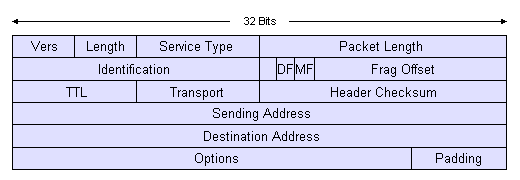
\includegraphics[width=1\textwidth]{IPv4HeaderImage}
    \caption{Formato dell'header IPv4}
     \label{fig:IPv4HeaderImage}
\end{figure}

I campi dell'header IP sono:
\begin{itemize}
\item \textbf{Version}, 4 bit indicanti la versione del protocollo IP del pacchetto; in IPv4 questo campo assume il valore 4.
\item \textbf{Internet Header Length} (IHL), 4 bit indicanti la lunghezza dell'header IP ( in word da 32 bit ); l'header pu� avere dimensione variabile a seconda se il campo \emph{Options} � settato o meno.
\item \textbf{Type of Service} (TOS), ottetto che nelle specifiche iniziali del protocollo ( RFC 791 ) davano la possibilit� all'host mittente di specificare il modo e la priorit� con cui il nodo destinatario doveva trattare il datagram. In realt� questo campo non � mai stato largamente utilizzato e negli ultimi e recentemente questi 8 bit sono stati ridefiniti e hanno la funzione di \emph{Differentiated services} (DiffServ) nell'IETF e \emph{Explicit Congestion Notification} (ECN) codepoints  (RFC 3168) necessari per le tecnologie basate su streaming in tempo reale come ad esempio per il \emph{Voice over IP} (VoIP).
\item \textbf{Total Length}, 16 bit, indica la dimensione massima in byte dell'intero dagram IP ( header e dati ); tale lunghezza pu� variare da un minimo di 20 byte (header minimo e senza alcun dato) a un massimo di 65535 byte. In ogni momento un host deve poter gestire datagrammi di dimensione minima 576 byte mente, se necessario, possono frammentare datagram di dimensione maggiore.
\item \textbf{Identification}, 16 bit, definito per identificare univocamente i vari frammenti in cui pu� essere suddiviso un datagram IP. Pu� essere anche utilizzato per valutare la presenza di datagram ridondanti ( indirizzo IP sorgente pi� Identification identificano univocamente un pacchetto ).
\item \textbf{Flags} ovvero 3 bit utilizzati per il controllo del protocollo e la frammentazione dei datagrammi. Il primo bit detto \emph{Reserved} � sempre settato a zero; vi sono poi DF (Don't Fragment) che se settato a 1 indica che il pacchetto non deve essere frammentato e MF (More Fragment) che se settato a 0 indica che � l'ultimo frammento ( o il solo frammento originario ) e tutti gli altri frammenti avranno quindi questo flag posto a 1.
\item \textbf{Fragment Offset}, 13 bit, indica l'offset, misurato in blocchi da 8 byte, di un particolare frammento relativamente all'inizio del datagram IP originario. L'offset massimo risulta pertanto essere 65526 byte che, sommato la dimensione dell'header IP, potrebbe eccedere la dimensione massima di 65535 byte prevista per un datagram IP.
\item \textbf{Time To Live} (TTL), 8 bit, indica il \emph{tempo di vita} di un pacchetto necessario per evitarne la persistenza indefinita sulla rete nel caso in cui non si riesca a recapitarlo al destinatario. Storicamente il TTL misurava i "secondi di vita" del pacchetto, mentre ora esso misura il numero di "salti" da nodo a nodo della rete: ogni router che riceve il pacchetto prima di inoltrarlo ne decrementa il TTL ( modificando quindi anche il campo Header Checksum ), quando questo arriva a zero il pacchetto non viene pi� inoltrato ma scartato. Tipicamente, quando un pacchetto viene scartato per esaurimento del TTL, viene automaticamente inviato un messaggio ICMP al mittente del pacchetto, specificando il codice di richiesta scaduta; la ricezione di questo messaggio ICMP � alla base del meccanismo di traceroute.
\item \textbf{Protocol}, 8 bit, indica il codice associato al protocollo utilizzato nel campo dati del pacchetto IP.
\item \textbf{Header Checksum}, 16 bit, � un campo usato per il controllo degli errori dell'header. Ad ogni hop, il checksum viene ricalcolato (secondo la definizione data in RFC 791) e confrontato con il valore di questo campo: se non c'� corrispondenza il pacchetto viene scartato. � da notare che non viene effettuato alcun controllo sulla presenza di errori nel campo Data deputandolo ai livelli superiori.
\item \textbf{Source Address}, 32 bit, indirizzo IP associato all'host del mittente del datagram.
\item \textbf{Destination Address}, 32 bit, indirizzo IP associato all'host del destinatario del datagram.
\item \textbf{Options} contiene opzione facoltative e poco usate per usi pi� specifici del protocollo. La dimensione del campo Options deve essere multipla di 32 bit altrimenti, per raggiungere tale scopo, vengono aggiunti dei bit privi di significato, \textbf{padding}.
\end{itemize}
\end{paragraph}
\end{subsection}
%NAT
\begin{subsection}{NAT}
NAT Network Address Translation � una tecnica che consente di mappare uno o pi� indirizzi IP di un \emph{address space} in un indirizzo IP appartenente a uno spazio di indirizzi diverso: questo avviene molto semplicemente modificando le informazioni sugli indirizzi di rete presenti in un datagram IP in transito su di un dispositivo di routing. Questa tecnica � stata originariamente pensata per semplificare le operazioni di rerouting del traffico IP in una rete senza rinumerare ciascun host di quella rete: ad esempio hosts appartenenti a una rete privata possono essere mappati su di un unico indirizzo IP appartenente a uno spazio di indirizzamento differente ( tendenzialmente un indirizzo IP pubblico ). Questo meccanismo viene realizzato memorizzando in un dispositivo di routing delle \emph{translation table} che mappano gli indirizzi IP non visibili dall'esterno in uno ( o pi� ) indirizzi IP pubblici modificando i datagram in uscita facendo sembrare dall'esterno che il mittente del pacchetto � il routing device. Quando viene ricevuto un pacchetto dall'esterno verso la rete interna privata il routing device, che mantiene le translation table, inoltrer� il pacchetto all'effettivo host destinatario. 
\\
Questa tecnica � molto utilizzata anche per preservare il consumo di indirizzi IPv4. Gli indirizzi IPv4 essendo formati da 32 bit possono generare un pool di 4.294.967.296 indirizzi: se si considerano i vari diversi indirizzi riservati e la sempre pi� diffusione di dispositivi che possono connettersi alla rete come laptop, smartphone e IoT questo pu� rappresentare un limite molto serio. Per tanto a partire dal 2004 � disponibile una nuova versione dell'internet protocol IPv6 che adotta indirizzi di dimensione pari a 128 bit. 
\end{subsection}
\begin{subsection}{ARP}
Il protocollo ARP (Address Resolution Protocol) � usato per determinare, dato un indirizzo IP, il corrispettivo indirizzo hardware di livello data-link. Quando un host vuole spedire un datagramma ad un altro nodo conoscendo il suo indirizzo IP ma non quello fisico, fa una richiesta ARP in broadcast sulla rete di appartenenza, chi ha l?indirizzo richiesto risponde con il proprio indirizzo MAC.
\\
Il corrispettivo protocollo ovvero che consente di risalire all'indirizzo IP di un host dato il suo MAC address � il protocollo RARP (Reverse Address Resolution Protocol).
\end{subsection}

%Frammentazione
\begin{subsection}{Frammentazione}
Per rendere il protocollo tollerante alle eventuali differenze di specifiche sottoreti � possibile effettuare la frammentazione dei datagram IP. In particolare ogni qual volta un datagram IP deve essere trasmesso attraverso un link con MTU (Maximum Transfer Unit, che rappresenta un limite superiore alla dimensione di un frame di livello data-link dipendente dall'hardware di rete) inferiore alla dimensione del pacchetto stesso questo verr� frammentato in pi� fragment che soddisfano il valore della MTU. Il router quindi prelever� il payload dal datagram IP e lo frammenter� in modo tale che il nuovo segmento dati pi� l'header IP possa essere contenuto come body di un frame di livello data-linke e facendo si che ogni payload del datagram abbia dimensione multipla di 8 byte ( campo Offset in header IP). In tutti i frammenti tranne l'ultimo inviato, che in genere avr� anche una dimensione minore rispetto ai precedenti, avranno il flag MF (More Fragment) settato a 1.
\end{subsection}

%Routing
\begin{subsection}{Routing}
Uno dei compiti caratteristici del livello rete � il \emph{routing} ovvero decidere su quale interfaccia di rete o porta inoltrare un pacchetto ricevuto verso la sua destinazione finale. In particolare i router mantengono delle tabelle di instradamento che possono essere popolate manualmente ( \emph{routing statico}, poco scalabile adatto esclusivamente per reti molto piccole ) o popolate da appositi protocolli di routing che mantengono le tabelle di routing aggiornate a seconda del variare della topologia della rete. Vi sono due tipologie principali di protocolli di routing: \emph{Distance Vector} e \emph{Link State}. Nel protocollo Distance Vector ogni router misura la distanza ( utilizzando una metrica che pu� tenere conto di diversi fattori ) dai nodi adiacenti tramite le informazioni ricevute dai nodi vicini. In un protocollo Link State, invece, ciascun nodo acquisisce informazione sullo stato dei collegamenti adiacenti e inoltra queste informazioni a tutti gli altri nodi sulla rete attraverso un pacchetto di tipo Link State trasmesso tramite un algoritmo di \emph{link state broadcast}.
\end{subsection}

\begin{subsection}{IPv6}
Internet Protocol version 6\cite{IPv6Bibliography} � la versione pi� recente dell'Internet Protocol formalizzato nel 1998 da IETF a seguito della recente crescita esponenziale dei dispositivi che accedono ad internet. IPv6 adotta indirizzi a 128 bit fornendo cos� $2^{128}$ indirizzi ovvero circa 3,4 x $10^{38}$ indirizzi. I protocolli IPv4 e IPv6 non sono stati progettati per essere interoperabili complicando cos� la transizione verso l'ultima versione dell'Internet Protocol seppure siano stati ideati dei meccanismi di transizione da un protocollo verso l'altro. Tuttavia la migrazione completa verso IPv6 dovrebbe venire nel 2025 con la deprecazione definitiva di IPv4.
\\
IPv6 oltre a estendere lo spazio di indirizzamento porta con se alcune nuove feature come la dimensione fissa dell'header a 40 byte, datagram non frammentabili dai router e la rimozione del checksum dall'header (ridondate in quanto presente in altri layer dello stack di rete).
Inoltre � stati aggiunto il supporto nativo alla sicurezza (IPsec) e inseriti meccanismi di autoconfigurazione come ad esempio ARP. 
\\
Gli indirizzi IPv6, composti da 128 bit, sono rappresentati come 8 gruppi di 4 cifre esadecimali ( 8 word di 16 bit ciascuna ) in cui le lettere vengono scritte in forma minuscola. Ad esempio fe80:0000:0000:0000:a4f5:f1ff:fe49:8d93 rappresenta un indirizzo IPv6 valido. In un indirizzo IPv6 una sequenza di zeri contigui composta da 2 o pi� gruppi pu� essere contratta con la semplice sequenza \emph{::} riducendo cos� l'indirizzo appena illustrato a fe80::a4f5:f1ff:fe49:8d93.

\begin{paragraph}{Datagram IPv6}
IPv6 specifica un nuovo header rispetto a IPv4 semplificandolo di molto eliminando alcuni campi poco usati e spostandoli in estensioni separate. Come gi� detto l'header IPv6 ha una dimensione fissa di 40 byte.

\begin{figure}[h]
    \centering
    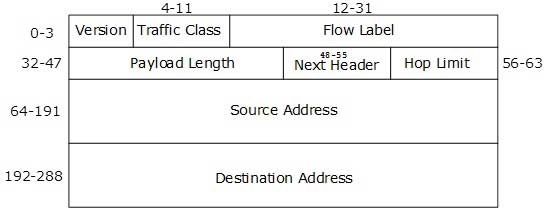
\includegraphics[width=1\textwidth]{IPv6HeaderImage}
    \caption{Header datagram IPv6}
     \label{fig:IPv6HeaderImage}
\end{figure}

In particolare eventuali estensioni vengono inviate successivamente: il campo \emph{next header} infatti definisce il tipo dell'header successivo nel caso siano inviate delle estensione altrimenti indica il protocollo del pacchetto incapsulato nel payload del datagram. �	quindi possibile avere pi� di un estensione per ciascun datagram.
Alcune tra le estensioni pi� comuni sono:
\begin{itemize}
\item \textbf{Hop-by-hop options} definisce un insieme arbitrario di opzioni intese per ogni hop attraversato.
\item \textbf{Routing packet} definisce un metodo per permettere al mittente di specificare la rotta da segure per un datagramma.
\item \textbf{Fragment packet} usato quando un datagramma viene frammentato.
\item \textbf{No next header} indica che i dati nel payload del datagramma non sono incapsulati in nessun altro protocollo.
\item \textbf{Destination options} definisce un insieme arbitrario di opzioni di interesse del solo destinatario.
\item \textbf{Mobility options} usato per Mobile IPv6.
\item \textbf{Altri protocolli (TCP, UDP, etc etc.)} indica il protocollo del pacchetto incapsulato nel payload.
\end{itemize}
\end{paragraph}
\end{subsection}
\begin{subsection}{Frammentazione in IPv6}
Come gi� brevemente accennato nell'ultima versione dell'Internet Protocol viene rimossa la frammentazione di una datagram IPv6 da parte dei router.
\\ 
\\
A differenza della versione 4 dell'Internet Protocol, in IPv6, la frammentazione avviene esclusivamente in maniera end-to-end ovvero ciascun datagram sar� frammentato dall'host sorgente e poi riassemblato dall'host destinatario senza ulteriore frammentazione da parte dei router intermedi.
\\
Rimuovendo la frammentazione da parte dei nodi intermedi di una trasmissione viene abbattuto l'overhead dovuto alla framentazione che era a carico dei router incrementando cos� il numero di pacchetti gestiti per unit� di tempo.
\\
Il protocollo IPv6 richiede che ogni link supporti la trasmissione di datagram di dimensione fino a 1280 byte.
\\
In caso di una frammentazione viene utilizzata l'estensione precedentemente accennata \emph{Fragment packet}. 
\\
Quando un host deve inviare un datagram IPv6 pu� valutare se tutti gli eventuali suoi frammenti abbiano una dimensione massima di 1280 byte oppure se utilizzare un algoritmo di discovery che gli consenta di scoprire qual � la dimensione minima supportata su uno dei link da attraversare per arrivare a destinazione. IETF suggerisce l'utilizzo del secondo approccio anche se questo potrebbe rappresentare un limite in quanto il percorso di ciascun datagram sarebbe ben definito e statico: nel caso un router non riesca per qualche motivo instradare il datagram su uno dei link predefiniti mander� un messaggio di errore all'host sorgente che calcoler� un nuove percorso.
\end{subsection}
\end{section}
%Transport Layer
\begin{section}{Transport Layer}
Il livello trasporto � il quarto livello dello stack di rete ISO/OSI che ha lo scopo di fornire un canale di comunicazione \emph{end-to-end} tra processi residenti in host diversi.
\\
Uno dei diversi protocolli di livello trasporto � il TCP (Transmission Control Protocol). TCP � un protocollo connection-oriented tramite il quale un flusso di dati inviato viene recapitato al destinatario senza errori. I frammenti dello stream vengono impacchettati e passati ai layer inferiori, sar� poi compito del ricevente provvedere a riassemblare ciascun pacchetto ed eventualmente, in caso di errori, chiederne il rinvio. TCP implementa inoltre un meccanismo per il \emph{flow control}, non permette cio� ad una sorgente "veloce" di congestionare un ricevente "lento", assieme al \emph{congestion control} che consente di evitare di congestionare i router che sono tra i due end-point.
\\
Considerato lo scenario e il contesto di questa tesi il protocollo di livello trasporto che pi� � degno di approfondimento � il protocollo UDP.
%UDP Protocol
\begin{paragraph}{Protocollo UDP}
Il protocollo UDP (User Datagram Protocol)\cite{UDPBibliography} � un protocollo di livello trasporto connection-less e best-effort cio� non assicura che un pacchetto sia effettivamente consegnato a destinazione. Applicazioni in esecuzione su host differenti possono scambiarsi messaggi, detti datagram, consegnandoli su appositi socket dedicati. Essendo un protocollo inaffidabile una volta inviato un datagram verso la rete l'applicazione sorgente non potr� mai sapere se effettivamente � stato consegnato a destinazione o meno. Ciascun datagram inviato � indipendente dai restanti datagram inviati ed inoltre non viene effettuata alcun tipo di frammentazione a livello trasporto. Non viene effettuato alcun tipo di controllo nemmeno per quanto riguarda l'ordine con cui i pacchetti vengono ricevuti dall'end-system. Tutti questi motivi UDP � un protocollo molto leggero e veloce ideale per applicazioni che necessitano di interattivit� cos� come ad esempio servizi di streaming audio/video in real-time. 
\\
L'header UDP, visti i pochi controlli di cui si fa carico il protocollo, risulta essere molto snello introducendo cos� un overhead molto basso.

\begin{figure}[h]
    \centering
    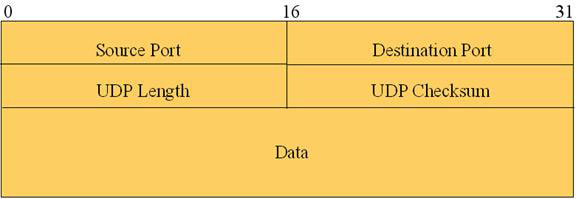
\includegraphics[width=1\textwidth]{UDPHeader}
    \caption{Header UDP}
     \label{fig:UDPHeaderImage}
\end{figure}

Nell'header UDP, oltre alle porte che indicano sostanzialmente le applicazioni (sorgente e destinataria) coinvolte nelle comunicazione, vi � il campo checksum. Questo campo � opzionale se la trasmissione avviene over IPv4 mentre obbligatorio se si utilizza IPv6 (header IPv6 non contiene campo sull'integrit� datagram).
\end{paragraph}
\end{section}
%Application Layer
\begin{section}{Application Layer}
Il livello applicazioni si colloca nella parte pi� alta dello stack ISO/OSI e coinvolge tutta una serie di protocolli che si occupano di fornire servizi per i processi delle applicazioni usate dagli utenti finali. I protocolli appartenenti a questo livello sono davvero numerosissimi e utilizzati dalle pi� disparate applicazioni come ad esempio FTP (File Transfer Protocol) o HTTP (HyperText Transfer Protocol) alla base del World Wide Web. 
\\
Se considerato il livello Application dello standard \emph{de jure} TCP/IP questo include anche i livelli presentazione e sessione del modello OSI.
Per quanto riguarda il livello applicazione si vuole ora approfondire i protocolli coinvolti nella tecnologia VoIP in quanto la applicazioni che sfruttano questa tecnologia possono toccare con mano l'oggetto di questa tesi.

%VoIP
\begin{subsection}{VoIP}
VoIP (Voice over IP)\cite{VoIPBibliography}  � una famiglia di tecnologie internet e protocolli di comunicazione per la distribuzione di comunicazioni vocali e sessioni multimediali attraverso il protocollo IP. 
\\
Il VoIP richiede due tipologie di protocolli di comunicazione in parallelo, una per il trasporto dei dati (pacchetti voce su IP), ed una per la segnalazione della conversazione che comprende la ricostruzione del frame audio, la sincronizzazione, l'identificazione del chiamante lo scambio di altri parametri di comunicazione cos� come indirizzp IP, porte e codec audio/video. 
\\
Per quanto riguarda la trasmissione dati la maggioranza delle implementazioni VoIP adottano il protocollo RTP (Real-time Transfer Protocol, basato su UDP). RTP viene usato assieme a RTPC (RTP Control Protocol) che monitora la \emph{qualit� del servizio} (QoS) inviando periodicamente delle statistiche ai partecipanti dello streaming multimediale senza per� trasportare alcun tipo di dato relativo alla comunicazione vera e propria. � stato inoltre definito SRTP (Secure Real-time Transfer Protocol) che introduce crittografia, autenticazione e integrit� in RTP.
\\
Per quanto concerne i protocolli di segnalazione, invece, nel corso degli anni ne sono stati sviluppati diversi. H.323\cite{Hdot323} definito dalla ITU-T (International Telecommunications Union) � stato uno dei primi protocolli pensati per il VoIP. H.323 nasce in ambito telefonico e delinea un'architettura completa per lo svolgimento di conferenze multimediali. Comprende la definizione dei formati di codifica a livello applicativo, la definizione dei formati per la segnalazione e il controllo, per il trasporto dei flussi multimediali ( audio, video e dati ). H.323 definisce anche alcuni meccanismi legati agli aspetti relativi alla sicurezza.
\\
Vi � poi SIP (Session Initiation Protocol)\cite{SIPBibliography} definito da IETF, operante a livello sessione del modello OSI, che gestisce in modo generale una sessione di comunicazione tra due o pi� entit�, ovvero fornisce meccanismi per instaurare, modificare e terminare (rilasciare) una sessione. Fornisce funzionalit� di instaurazione e terminazione di una sessione, operazioni di segnalazione , tono di chiamata, chiamata in attesa, identificazione del chiamante e molto altro ancora. Adotta un un pattern message/response e i messaggi principali di SIP sono:
\begin{itemize}
\item REGISTER, inviato da un client verso un server SIP che mantiene una mappa degli utenti SIP e la loro posizione (indirizzi IP).
\item INVITE, utilizzato per inizializzare una sessione di comunicazione specificando l'identificativo dell'utente con la quale si vuole comunicare; inviato da un client verso un server SIP che risponde con l'indirizzo dell'altro end-node con la quale si vuole avviare la sessione assieme ad altri parametri di configurazione.
\item re-INVITE, viene utilizzato quando uno dei parametri di configurazione cambia (ad esempio l'indirizzo IP).
\end{itemize}
SIP � pi� recente e viene largamente utilizzando riscontrando un maggiore successo di H.323.
\end{subsection}

\end{section}
\end{chapter}
%\end{document}
\documentclass[12pt,a4paper,openright,twoside]{book}
\usepackage[italian]{babel}
\usepackage[latin1]{inputenc}
\usepackage{fancyhdr}
\usepackage{indentfirst}
\usepackage{graphicx}
\graphicspath{ {Images/}  }
\usepackage{newlfont}
\usepackage{amssymb}
\usepackage{amsmath}
\usepackage{latexsym}
\usepackage{amsthm}


\pagestyle{fancy}\addtolength{\headwidth}{20pt}
\renewcommand{\chaptermark}[1]{\markboth{\thechapter.\ #1}{}}
\renewcommand{\sectionmark}[1]{\markright{\thesection \ #1}{}}
\rhead[\fancyplain{}{\bfseries\leftmark}]{\fancyplain{}{\bfseries\thepage}}
\cfoot{}

\linespread{1.3}  

\begin{document}
\begin{chapter}{Architettura}
Tutti i dispositivi mobili attualmente offrono diverse modalit� di accesso ad internet basti pensare a uno smartphone che consente l'accesso a internet sia in modalit� Wi-Fi che attraverso la telefonia mobile con la tecnologia 3G fino alla pi� recente tecnologia 4G.
\\
In questo capitolo si vuole descrivere un'architettura che consente a un user app che fornisce un servizio multimediale in esecuzione su di un mobile device \emph{multi-homed}, ovvero che monta pi� di un'interfaccia di rete, di sfruttare tutte le sue NIC (Network Interface Card). In particolare un servizio multimediale ( come pu� essere una trasmissione audio o video ) viene solitamente realizzato tramite protocollo UDP: l'architettura presentata in questo capitolo fornisce un meccanismo in grado da rendere possibile l'inoltro di ciascun datagram UDP attraverso l'interfaccia di rete pi� adatta al momento della trasmissione. Questa architettura � detta ABPS ( Always Best Packet Switching ) ma prima di descriverne i suoi principali aspetti verr� descritto lo stato dell'arte per quel che riguarda la gestione della mobilit� dei nodi mobili.

\begin{section}{Seamless Host Mobility \& State Of the Art}
Nel corso degli ultimi anni sono state sviluppate diverse architetture che consentono a un nodo mobile in movimento di avere accesso continuo a servizi di rete in particolare sono stati sviluppati diversi approcci che cercano di far si che device che montano pi� interfacce di rete possano effettuare un \emph{handover} da un interfaccia di rete all'altra in maniera del tutto trasparente all'app utente in esecuzione, \emph{seamless}. 
Per handover o handoff si intende il processo di cambio di interfaccia di telecomunicazione da parte di un dispositivo multi-homed (\emph{vertical handoff}) oppure il cambio di punto di accesso mantenendo la stessa tecnologia (\emph{horizontal handoff}, ad esempio cambio di AP all'interno di una stessa rete WLAN).
\\
In generale un'architettura per la seamless mobility dovrebbe essere responsabile di identificare univocamente ciascun nodo mobile, permettere a un nodo mobile di essere raggiungibile dall'altro nodo coinvolto nella comunicazione (Correspondent Node) che pu� anch'esso essere un nodo mobile e dovrebbe monitorare la QoS fornita dalle diverse reti a cui il nodo mobile potrebbe connettersi in modo da prevedere la necessit� di un handoff ed eventualmente, quindi, il cambio di interfaccia di rete e quindi effettuare l'handoff in maniera \emph{seamless} assicurando la continuit� della comunicazione.
\\
Vediamo ora una rassegna di tutte le soluzioni sviluppate finora per implementare meccanismi di seamless handoff in un contesto di un nodo mobile che attraversa reti eterogenee. 
% K. Kong et al, ?Mobility management for All-IP mobile networks: Mobile IPv6 vs. Proxy Mobile IPv6?, IEEE Wireless Communications, April 2008.
\begin{paragraph}{Implementazioni a livello network}
Tra le architetture presenti che lavorano a livello network vi � Mobile IP version 6 e le sue ottimizzazioni come ad esempio FMIP (Fast Handover Mobile IPv6), HMIP (Hierarchical Mobile IPv6) e PMIP (Proxy Mobile IPv6). Tutte queste architetture adottano un \emph{Home Agent} ovvero un'entit� aggiuntiva che opera all'interno della rete alla quale il nodo mobile appartiene. L'home agent ricopre il ruolo di \emph{location registry} ovvero un servizio \emph{always on}: quando un nodo mobile cambia interfaccia di rete e quindi indirizzo IP lo comunica al location registry (\emph{registration phase}) che tiene una mappa degli indirizzi. Quando un Correspondent Node vuole comunicare con il nodo mobile invia al location registry una \emph{lookup phase} per ottenere l'indirizzo corrente del mobile node. Tutti i nodi coinvolti devono avere il supporto a IPv6: in particolare l'indirizzo attuale e l'identificativo univoco del nodo mobile sono trasmessi attraverso delle estensioni di IPv6. Il fatto che tutti i nodi debbano necessariamente supportare IPv6 rappresenta un limite di questo approccio architetturale. Un altro limite di questo approccio � che presso un home agent pu� essere registrato l'indirizzo di una sola interfaccia di rete per ogni nodo impedendo cos� un supporto al multihoming visto che la latenza introdotta dai numerosi messaggi di autenticazione procurerebbe un overhead insostenibile per la tipologia di comunicazione multimediale che dovrebbe essere veloce e snella.
\end{paragraph}
\begin{paragraph}{Implementazioni tra livello rete e trasporto}
Esistono alcune possibili implementazioni di architetture per la seamless host mobility che introducono un nuovo layer posto tra il livello rete e quello trasporto: questa nuova astrazione dovr� essere aggiunta su tutti i nodi prendenti parte alla comunicazione. Alcuni esempi possono essere HIP (Host Identity Protocol) e LIN6 (Location Independet Addressing for IPv6). Il location registry si comporta in maniera simile a un server DNS mappando l'identificativo di un host e la sua attuale posizione restando per� all'esterno della rete di appartenenza del nodo mobile. Un limite di questo approccio � nella necessit� di modificare lo stack di rete di tutti i nodi coinvolti.
\end{paragraph}
\begin{paragraph}{Implementazioni a livello trasporto}
Vi sono alcuni protocolli che operano a livello trasporto: ogni nodo coinvolto in una comunicazione si comporta in maniera pro-attiva fungendo da location registry informando direttamente il proprio Correspondent Node ogni qualvolta la configurazione di rete cambia. Il limite di questo approccio sta nel fatto che se entrambi i mobile end-system cambiano contemporaneamente gli indirizzi IP a seguito di un handoff diventano mutuamente irraggiungibili. Inoltre, come nel precedente approccio, questo tipo di architettura richiederebbe una modifica delle applicazioni sia sul nodo mobile che sul suo correspondent node.
\end{paragraph}
\begin{paragraph}{Implementazioni a livello Sessione}
Sono state progettato alcune soluzioni che operano a livello sessione come ad esempio TMSP (Terminal Mobility Support Protocol) che sfrutta un SIP server ausiliario collocato fuori dalla rete di un nodo mobile che funge da location registry che mappa ciascun identificativo SIP di utente al suo indirizzo IP attuale. Ogni nodo mobile esegue un client SIP che manda un messaggio di tipo REGISTER per aggiornare il suo indirizzo IP. I messaggi INVITE, al solito, sono utilizzati per avviare comunicazioni con altri nodi cos� come i messaggi di tipo re-INVITE.
Gli approcci operanti a livello Session non sembrano essere particolarmente efficienti per i ritardi introdotti dal pattern message/response dei sistemi basati SIP.
%The session-layer solutions seem to be not efficient as they invoke an external localization service when an IP reconfiguration occurs. In particular, the SIP-based services introduce an additional delay due to their message/response behavior; in case of reconfiguration the MN interrupts the communication, sends a SIP signaling message to the CN and waits for the response before resuming the transmission. With this in view, the IHMAS work presented in [6] provides a solution to minimize handoff delays by exploiting a SIP-based, IMS compliant proactive mechanism that performs registration and renegotiation phases for novel connections while keeping the media flows active over old connections, if these are available.
\end{paragraph}
\end{section}
\begin{section}{Always Best Packet Switching}
Un'architettura progettata all'interno del Dipartimento di Informatica dell'Universit� di Bologna che supera i limiti delle implementazioni precedentemente descritte � ABPS (Always Best Packet Switching).
L'architettura ABPS � composta da due componenti principale:
\begin{itemize}
\item \textbf{fixed proxy server}, una macchina esterna alla rete in cui si trova il mobile node; munito di IP pubblico statico e fuori da qualsiasi firewall o NAT. Il fixed proxy server gestisce e mantiene tutte le comunicazione da un mobile node verso l'esterno e viceversa: nel caso di un handoff e quindi di una riconfigurazione delle interfacce di rete del nodo mobile il fixed proxy server nasconde questi cambiamenti al correspondent node facendo si che la comunicazione continui in maniera del tutto trasparente.
\item \textbf{proxy client}, in esecuzione su ogni mobile node, mantiene per ogni NIC una connessione verso il fixed proxy server. Applicazioni in esecuzioni su un mobile node possono quindi sfruttare un multi-path virtuale creato tra il proxy client e il fixed proxy server per comunicare con il resto del mondo.
\end{itemize}

\end{section}
\end{chapter}

\end{document}
\documentclass[12pt,a4paper,openright,twoside]{book}
\usepackage[italian]{babel}
\usepackage[latin1]{inputenc}
\usepackage{fancyhdr}
\usepackage{indentfirst}
\usepackage{graphicx}
\graphicspath{ {Images/}  }
\usepackage{newlfont}
\usepackage{amssymb}
\usepackage{amsmath}
\usepackage{latexsym}
\usepackage{amsthm}
\usepackage{listings}

\pagestyle{fancy}\addtolength{\headwidth}{20pt}
\renewcommand{\chaptermark}[1]{\markboth{\thechapter.\ #1}{}}
\renewcommand{\sectionmark}[1]{\markright{\thesection \ #1}{}}
\rhead[\fancyplain{}{\bfseries\leftmark}]{\fancyplain{}{\bfseries\thepage}}
\cfoot{}
\linespread{1.3}  
\begin{document}

\begin{chapter}{Transmission Error Detector}
In questo capitolo si vuole illustrare le fasi di progettazione e implementazione di un modulo TED per ABPS per kernel Linux 4.0.
Nel precedente capito si � descritto brevemente il funzionamento di TED e il suo funzionamento nel sistema ABPS pensato per il supporto alla mobilit�.
\\
Il meccanismo di Transmission Error Detection pu� essere applicato a qualsiasi interfaccia di rete di un dispositivo mobile. In questa capitolo verr� illustrata la progettazione di un modulo TED per Wi-Fi.
\\
Transmission Error Detector � implementato in maniera \emph{cross-layer} lungo lo stack di rete del kernel Linux e ha lo scopo di monitorare ciascun datagram UDP in invio da una certa interfaccia di rete e notificare ad un eventuale ABPS proxy client lo stato di consegna del pacchetto all'access point. Per far ci� TED introduce una notifica di tipo \emph{First-hop Transmission Notification} che sar� fatta pervenire al proxy client.
\\
Per monitorare uno specifico datagram il proxy client necessit� di un identificativo che identifichi univocamente un dato datagram. A tal proposito si � estesa la system call \emph{sendmsg} in modo tale che ritorni un id univoco per il messaggio appena spedito.  
\begin{section}{Progettazione e implementazione}
Transmission Error Detector opera su pi� layer dello stack di rete del kernel Linux e ha il compito di monitorare ciascun datagram trasmesso da un proxy client ABPS e notificarne lo stato di consegna in modo tale da poter valutare la QoS di quel collegamento ed eventualmente inoltrare quello stesso datagram attraverso un'altra NIC del nodo mobile.
\\
Come gi� precedentemente accennato TED � implementato in maniera cross-layer su pi� livelli dello stack di rete del kernel di Linux.
\begin{subsection}{Livello trasporto}
Le applicazioni per le quali ABPS vuole essere un supporto alla mobilit� sono le applicazioni multimedia-oriented che come gi� trattato nei capitoli precedenti sono solitamente progettate per utilizzare UDP. Un'applicazione che utilizza UDP per le sue comunicazioni di rete sfrutta uno o pi� socket datagram ovvero di tipo connectionless.
\\
Per poter valutare la ritrasmissione di un dato messaggio il proxy client necessita di un meccanismo di identificazione per ciascun datagram. A tal proposito si � esteso la system call \emph{sendmsg} in modo tale che possa ritornare un \textbf{id} univoco per il messaggio in invio cosicch� il proxy client possa mantenerlo e usarlo per riferirsi a quel preciso datagram. Tutte le notifiche ricevute poi in seguito dal proxy client e provenienti da TED faranno riferimento a un datagram utilizzando lo stesso identificativo. 
\\
La system call sendmsg consente di inviare, assieme al contenuto del messaggio, delle informazioni di controllo aggiuntive dette \emph{ancillary data} che non saranno per� trasmesse lungo la rete. Dal punto di vista implementativo i dati di tipo ancillary sono realizzati in POSIX tramite una sequenza di strutture \textbf{struct cmsghdr} contenenti le informazioni di controllo. L'estensione di sendmsg in particolare prevede l'utilizzo di ancillary data in fase di invio:
\begin{itemize}
\item Per segnalare a TED che l'app invocante la system call sendmsg richiede di poter ricevere l'id per il messaggio in invio. Per far ci� viene introdotto un nuovo valore non utilizzato per il campo \textbf{cmsg\_type} della struct cmsghdr.
\item Per passare a TED un'indirizzo di memoria in user space dove TED potr� assegnare l'id generata per il datagram in invio.
\end{itemize}

\end{subsection}


\end{section}

\end{chapter}
\end{document}
%\documentclass[12pt,a4paper,openright,twoside]{book}
%\usepackage[italian]{babel}
%\usepackage[latin1]{inputenc}
%\usepackage{fancyhdr}
%\usepackage{indentfirst}
%\usepackage{graphicx}
%\usepackage{newlfont}
%\usepackage{amssymb}
%\usepackage{amsmath}
%\usepackage{latexsym}
%\usepackage{amsthm}
%
%\pagestyle{fancy}\addtolength{\headwidth}{20pt}
%\renewcommand{\chaptermark}[1]{\markboth{\thechapter.\ #1}{}}
%\renewcommand{\sectionmark}[1]{\markright{\thesection \ #1}{}}
%\rhead[\fancyplain{}{\bfseries\leftmark}]{\fancyplain{}{\bfseries\thepage}}
%\cfoot{}
%
%\linespread{1.3}  
%
%\begin{document}
%        \begin{chapter}{Test \& valutazioni sperimentali}
%        \usepackage[italian]{babel}
%        \usepackage[latin1]{inputenc}
%        \usepackage{fancyhdr}
%        \usepackage{indentfirst}
%        \usepackage{graphicx}
%        \usepackage{newlfont}
%        \usepackage{amssymb}
%        \usepackage{amsmath}
%        \usepackage{latexsym}
%        \usepackage{amsthm}
%        
%        \pagestyle{fancy}\addtolength{\headwidth}{20pt}
%        \renewcommand{\chaptermark}[1]{\markboth{\thechapter.\ #1}{}}
%        \renewcommand{\sectionmark}[1]{\markright{\thesection \ #1}{}}
%        \rhead[\fancyplain{}{\bfseries\leftmark}]{\fancyplain{}{\bfseries\thepage}}
%        \cfoot{}

%\linespread{1.3}  
%TEST E VALUTAZIONI SPERIMENTALI}

\begin{chapter}{Test \& valutazioni sperimentali}

Dopo aver illustrato il funzionamento e l'implementazione del TED, passiamo ora ad analizzare i dati relativi alla trasmissione di pacchetti tramite la nostra applicazione.
Lo scopo dei test effettuati � quello di analizzare la QoS del segnale e come pu� variare in diversi scenari.
Questo ci � utile in quanto, in base ai risultati ottenuti, si pu� decidere se cambiare NIC per l'invio di determinati pacchetti.


Per poter analizzare 




\begin{section}{Raccolta dati}
Andremo ora a mostrare quali test sono stati effettuati. In particolare mostreremo quali dispositivi sono stati utilizzati per fare le prove, i parametri di valutazione ed i risultati ottenuti.

 
\begin{subsection}{Dispositivi}
Per effettuare delle prove sperimentali, sono stati utilizzati diversi dispositivi. In particolare due per simulare il client ( o nodo mobile ) ed altri per creare traffico nella rete, in modo da impegnare il canale per avere condizioni simili ad un tipico scenario di utilizzo.
Per ogni dispositivo � interessante mostrare per cosa � stato utilizzato. Nel caso di un nodo della rete, mostreremo anche il sistema operativo, il kernel, il processore e scheda di rete.




\begin{paragraph}{ZyXEL NBG4615 v2}
Access point utilizzato durante i test. � stata impostata la modalit� Wi-Fi 802.11b/g/n.

\end{paragraph}


\begin{paragraph}{LB-LINK BL-WN151}
Adattatore Wireless USB. Velocit� fino a 150Mb/s, supporta 802.11b/g/n.
� stata utilizzata principalmente sui Raspberry, visto che non dispongono di wireless integrato.
\end{paragraph}

\begin{paragraph}{NETGEAR WG111}
Adattatore Wireless USB. Velocit� fino a 54Mb/s, supporta 802.11b/g.
Questo adattatore � pi� lento ed � stato usato sul computer HP quando il wireless integrato dava dei problemi. 

\end{paragraph}

\begin{paragraph}{HP Pavilion dv6 Entertainment PC}
Questo notebook � stato utilizzato come client. Abbiamo montato un kernel versione 4.0.1, modificato tramite la procedura illustrata precedentemente. 
Le specifiche tecniche sono: 
\begin{itemize}
 \item Kernel: Linux versione 4.0.1 modificata.
 \item Processore: Intel Core i5 CPU M 430.
 \item Sistema operativo: Ubuntu 14.04 LTS 64-bit.
 \item Scheda di rete: Broadcom BCM43225 802.11b/g/n.
\end{itemize}

\end{paragraph}

\begin{paragraph}{DELL Latitude E6400}
Anche questo notebook � stato utilizzato come client, e vi � quindi montato un kernel versione 4.0.1 modificato. 
Le specifiche tecniche sono: 
\begin{itemize}
 \item Kernel: Linux versione 4.0.1 modificata.
 \item Processore: Intel Core 2 Duo.
 \item Sistema operativo: Ubuntu 14.04 LTS 32-bit.
 \item Scheda di rete: Intel Corporation WiFi Link 5100 802.11a/g/n.
\end{itemize}

\end{paragraph}


\begin{paragraph}{Raspberry Pi Model 2}
Abbiamo utilizzato questo raspberry per creare traffico sulla rete.
Le specifiche tecniche sono: 
\begin{itemize}
 \item Kernel: Linux versione 3.18.0-20-rpi2.
 \item Processore: 900MHz quad-core ARM Cortex-A7.
 \item Sistema operativo: Raspbian.
 
\end{itemize}

\end{paragraph}


\begin{paragraph}{UDOO Quad}
Abbiamo utilizzato la UDOO per creare traffico sulla rete, insieme ad i raspberry.
Le specifiche tecniche sono: 
\begin{itemize}
 \item Kernel: Kernel Linux 3.0.35.
 \item Processore: Freescale i.MX 6 ARM Cortex-A9 CPU Dual/Quad core 1GHz.
 \item Sistema operativo: UDOObuntu.
 
\end{itemize}

\end{paragraph}



\begin{paragraph}{Raspberry Pi Model B}
Abbiamo utilizzato questo raspberry per creare traffico sulla rete, ma a volte � stato anche utilizzato come server.
Le specifiche tecniche sono: 
\begin{itemize}
 \item Kernel: Kernel Linux 3.18.7+.
 \item Processore: 700 MHz single-core ARM1176JZF-S.
 \item Sistema operativo: Raspbian Wheezy.
\\ 
\end{itemize}

\end{paragraph}


\end{subsection}




\begin{subsection}{Parametri di valutazione}
Per poter analizzare i test in modo ottimale e per avere dei dati su cui lavorare abbiamo deciso di controllare alcuni parametri.
\\
I parametri che ci interessano maggiormente sono:

\begin{itemize}
 \item \textbf{ACK}: se � stato ricevuto un ACK o un NACK da parte dell'AP. 
 \item \textbf{Data}: � dato dalla data e dall'orario di invio del pacchetto.
 \item \textbf{Tempo}: � il tempo in millisecondi tra l'invio del pacchetto e la ricezione della notifica da parte dell'access point.
 \item \textbf{Retry count}: � il numero di tentativi di invio di un determinato pacchetto.
 \item \textbf{Versione IP}: IPv4 o IPv6.
 \item \textbf{Configurazione}: � la configurazione dei dispositivi utilizzati durante l'esperimento.
 \item \textbf{Wait}: indica se la recv � bloccante.
 
\end{itemize}
Abbiamo scelto questi parametri perch� ci permettono di poter giudicare in maniera chiara l'andamento dei pacchetti e la situazione della rete.
In particolare sono molto significativi il tempo, l'ACK ed il retry count.
Grazie a questi dati si pu� analizzare in modo dettagliato la situazione di ogni singolo pacchetto. L'applicazione pu� leggere l'ACK e successivamente decidere di rimandare il pacchetto in base ai millisecondi passati prima di ricevere la notifica.
Il numero di retry count risulta rilevante per confrontare differenti situazioni di traffico, oppure per notare cosa succede in caso di trasmissione in movimento.


Gli altri parametri che abbiamo deciso di utilizzare hanno un valore pi� trascurabile per un singolo pacchetto, ma possono diventare eloquenti per analizzare i dati a posteriori.
In particolare si potrebbe notare in base all'orario se c'� un evidente rallentamento della trasmissione. Ad esempio si potrebbe notare come in una zona industriale la QoS migliori durante la sera/notte.


Un altro dato che pu� essere utilizzato per esaminare i dati raccolti � la versione IP, si pu� controllare se c'� un differenza notevole tra IPv6 e IPv4 a parit� di condizioni.


Le configurazioni, invece, riguardano i dispositivi utilizzati durante un test e lo scenario applicativo. Andremo a mostrare quali configurazioni sono state provate in modo pi� dettagliato successivamente.
Per quanto riguarda la wait abbiamo deciso di fare sia una recv bloccante che una non bloccante. Abbiamo fatto dei test con entrambe e abbiamo analizzato le differenze, che andremo a descrivere pi� avanti.

Si potrebbero utilizzare anche altre informazioni ( ad esempio la bitrate ) per analizzare meglio i risultati, che saranno approfondite negli sviluppi futuri.








\end{subsection}

\begin{subsection}{Configurazioni}
Per ottenere dei risultati che potessero rispecchiare un reale utilizzo da parte di un nodo mobile abbiamo creato diverse configurazioni di dispositivi.
In particolare abbiamo deciso di tenere conto di alcuni possibili scenari di utilizzo, che sono:
\begin{itemize}
 \item Dispositivo client in movimento oppure fermo.
 \item Utilizzo indoor o outdoor.
 \item Trasmissione in linea diretta oppure trasmissione con un ostacolo tra nodo mobile ed AP.
 \item Assenza di traffico sulla rete in contrapposizione ad uno o pi� hosts wireless a creare traffico.
 \item In caso di presenza di nodi sulla rete abbiamo utilizzato anche la distanza e la velocit� come parametri.
 \item Trasmissioni ad un host della stessa sottorete oppure ad una rete esterna.
 \item Dimensione dei pacchetti.
\end{itemize}
Dati questi possibili utilizzi, abbiamo creato alcune configurazioni per valutare la qualit� del collegamento.
Il nostro interesse si � focalizzato sulla costruzione di un prodotto cartesiano tra tutte le opzioni.
Abbiamo quindi provato col nodo mobile fermo, da solo nella rete ed in linea diretta con l'AP.
In questa configurazione abbiamo anche valutato le possibili differenze in velocit� tra recv bloccante e non bloccante. La scelta tra queste due opzioni � stata implementata nell'applicazione di prova che abbiamo creato e che abbiamo descritto precedentemente.
\\
In contrapposizione a questa prima configurazione, abbiamo testato un nodo mobile solitario nella rete, fermo ma con un ostacolo tra lui e l'AP. Come ostacolo � stato scelto un muro, di larghezza di circa 15 centimetri.
\\
Per completare la raccolta dati da analizzare abbiamo fatto altre due configurazioni, andando a modificare quelle precedenti usando il nodo mobile in movimento.
\\
Queste prime configurazioni ci permettono gi� di raccogliere importanti dati, che per� non possono riflettere un reale utilizzo di una applicazione.
Questo perch� difficilmente la trasmissione VoIP avverr� con il dispositivo da solo sulla rete, ma la rete potr� essere pi� o meno congestionata in base al luogo o all'orario.
\\
Per rispondere a questa esigenza abbiamo deciso di fare delle prove con uno o pi� host attivi sulla rete, in modo che andassero a causare traffico per rallentare il nodo mobile.
\\
Abbiamo quindi creato altre configurazioni, andando in ognuna a modificare il numero di hosts ed altri parametri. Per quanto riguarda gli host li abbiamo lasciati sempre fermi, ma abbiamo modificato la distanza in diverse prove.
In questo modo gli host trasmetteranno pi� o meno velocemente e vogliamo andare a verificare al client dia pi� fastidio avere host lenti o veloci. Per controllare le velocit� � stata creata una applicazione in grado di stabilire la bitrate. Questa applicazione sar� descritta successivamente.


Analizziamo ora i settaggi che sono stati implementati.
In particolare avremo il nodo mobile fermo ed un host attivo, entrambi in linea diretta con l'access point. Da questa configurazione base abbiamo allontanato l'host, fino a variare la velocit� in modo significativo ( anche di un fattore 1/20 ).
\\
Queste ultime configurazione sono state ampliate anche con l'uso della recv prima bloccante, e poi non bloccante.
Invece per quanto riguarda tutte le configurazioni a seguire abbiamo deciso di testare l'applicazione solo con la modalit� della recv non bloccante. 
Questo � stato fatto perch� i primi dati empirici erano stati raccolti in quel modo e non si voleva quindi andare ad alterare il risultato.
Avendo comunque analizzato separatamente il comportamento bloccante e non, possiamo dare una congettura di quello che pu� succedere in caso di comportamento non bloccante.
\\
Anche in questo caso, per ogni configurazione creata, ne abbiamo create altre in cui abbiamo scelto parametri diversi.
Quindi per ognuna � stata tenuta una determinata struttura e siamo andati a modificare un parametro alla volta, registrato tutti i dati ottenuti.
\\
Le configurazioni che useremo nel corso delle valutazioni dei risultati sono descritte in appendice.

\end{subsection}




\begin{subsection}{Dettagli implementativi}
Avendo descritto quali parametri e quali configurazioni abbiamo descritto, ci concentriamo ora sulla parte implementativa dei test.
I principali problemi da risolvere in questa parte erano:
\begin{itemize}
 \item Velocit� degli hosts.
 \item Salvataggio dei dati.
 \item Elaborazione dei dati.
\end{itemize}
Per quanto riguarda la misurazione della velocit� degli hosts, abbiamo creato una semplice applicazione che vada a misurarla.
Per realizzarla abbiamo creato una connessione tra due hosts, un client ed un server.
Abbiamo scelto di realizzare la applicazione tramite socket TCP; � stata comunque implementata anche la versione UDP. 
\\
Il client trasmette un file tramite Wi-Fi ed il server si mette in ascolto e calcola la velocit� del client.
Il server � stato collegato all'AP tramite ethernet, e non wireless, per evitare di introdurre eventuali ritardi ed incognite.
Queste misurazioni sono state fatte all'interno della stessa sottorete, per non influenzare i risultati con la velocit� della linea ADSL.
Nel server il calcolo � stato realizzato tramite la divisione tra il totale dei bit ricevuti e i secondi necessari per la ricezione.
Il totale dei bit � stato semplicemente ricavato dal totale di tutti i Byte ricevuti, moltiplicati per 8.
I secondi, invece, sono stati ottenuti catturando il tempo prima dell'inizio della ricezione e appena finita la ricezione ( tramite la \emph{time(NULL)} ).
Successivamente � stata fatta la differenza tra i due time ed � stata calcolata la velocit� in Mb/s.
Successivamente, alla fine della ricezione di tutti i Byte, � stato catturato il tempo.
\\
La velocit� che � stata rilevata non pu� essere considerata perfetta in quanto ci potrebbero alcuni fattori che possono andare ad alterarla. 
Possiamo per� darla per buona perch�, per ogni host, � stata misurata pi� volte ed � stata successivamente scelta la media. 
Inoltre � stata misurata, nella maggior parte dei casi, in una zona poco abitata e di sera o notte, quindi l'interferenza data da altri dispositivi era minima.
\\

Per quanta riguarda il salvataggio dei dati, abbiamo scelto di farlo in un file in formato \emph{JSON}.
Abbiamo scelto il JSON per la facilit� di leggere i dati salvati. I dati sono stati salvati come un array di pacchetti, e per ogni pacchetto � stato salvato:
\begin{itemize}
 \item id del pacchetto.
 \item millisecondi tra invio pacchetto e ricezione della notifica.
 \item numero di tentativi di invio.
 \item versione IP.
 \item boolean per ack.
 \item numero della configurazione.
 \item data.
 
\end{itemize}
I dati salvati sono i parametri di valutazione che abbiamo precedentemente scelto.
Per utilizzare il JSON all'interno di C abbiamo incluso una apposita libreria, la \emph{json/json.h}.
\\
Un esempio di file JSON � il seguente:



\begin{lstlisting}[language=json,firstnumber=1]
{ "pacchetti": [ 

	{ "testId": 4713, "type": 6, "ack": true, "time": 0, "retrycount": 0, "ipVersion": "ipv6", "date": "Sat Jun 20 22:53:38 2015\n" },
	{ "testId": 4714, "type": 6, "ack": true, "time": 6, "retrycount": 0, "ipVersion": "ipv6", "date": "Sat Jun 20 22:53:38 2015\n" },
	{ "testId": 4715, "type": 6, "ack": true, "time": 4, "retrycount": 0, "ipVersion": "ipv6", "date": "Sat Jun 20 22:53:38 2015\n" },
	{ "testId": 4716, "type": 6, "ack": true, "time": 11, "retrycount": 0, "ipVersion": "ipv6", "date": "Sat Jun 20 22:53:38 2015\n" },
	{ "testId": 4717, "type": 6, "ack": true, "time": 0, "retrycount": 0, "ipVersion": "ipv6", "date": "Sat Jun 20 22:53:38 2015\n" },
	{ "testId": 4718, "type": 6, "ack": true, "time": 6, "retrycount": 0, "ipVersion": "ipv6", "date": "Sat Jun 20 22:53:38 2015\n" }
  ]
}


\end{lstlisting}


Grazie all'utilizzo di un file JSON per il salvataggio dei dati, ne risulta pi� semplice l'analisi.
Per poter elaborare i dati abbiamo scelto di creare vari script utilizzando il linguaggio \emph{Python}. 
� stato scelto il Python perch� supporta il JSON e perch� permette di effettuare tutte le operazioni necessarie in poche righe.
\\
Sono stati realizzati diversi script per svolgere diversi compiti. Ogni script ha uno scopo specifico ( ad esempio calcolare la media dei tempi di notifica, oppure il numero di nack ricevuti ).
Ad ogni script, a meno di casi particolari, viene passato il file JSON ed il numero di configurazione.
Ognuno di questi script andr� ad aprire il file di log, nel quale sono salvati tutti i dati.
Una volta aperto, viene convertito in una serie di elementi di un array JSON.
Ora, grazie alla configurazione passato da comando, sar� possibile andare ad analizzare i dati.
Ad esempio, il file Python per calcolare la media dei tempi di notifica di una certa configurazione �:


\begin{lstlisting}[language=python]
#!/usr/bin/python
# -*- coding: UTF-8 -*-
# all_avg_time.py
import json
import sys

tipo=-1
nPkt=0
numRetry=0
try:
	inputFile=sys.argv[1]
	tipo=int(sys.argv[2])
except:
	sys.exit("missing argument")

with open(inputFile) as data_file:    
    data = json.load(data_file)

for el in data["pacchetti"]:
	if el['type']==tipo:
		if el['ack']== True :
			numRetry=numRetry+el['retrycount']
			nPkt=nPkt+1	
	
avg=float(numRetry)/float(nPkt)
print(avg)


\end{lstlisting}

Sfruttando gli script che abbiamo realizzato siamo in grado di esprimere delle valutazioni su ogni aspetto che volevamo prendere in considerazione.


\end{subsection}


\begin{subsection}{Test effettuati}
Per effettuare i test ci siamo basati sui parametri e sulle configurazioni scelti precedentemente. 
La disposizione tipica della rete � quella in figura~\ref{fig:salaMengo}.


\begin{figure}[h]
    \centering
    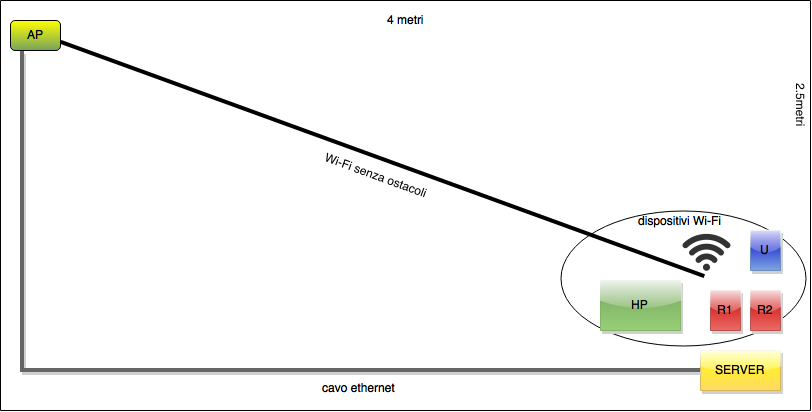
\includegraphics[width=1\textwidth]{salaMengo}
    \caption{Disposizione dei dispositivi maggiormente utilizzata. R1 ed R2 sono i Raspberry, mentre U � la UDOO.}
     \label{fig:salaMengo}
\end{figure}

In particolare, � stato usato il computer HP per svolgere la maggior parte dei test. 
Per creare del traffico in rete, invece, sono stati generalmente utilizzati il Raspberry Pi 2, la UDOO ed il Raspberry Model B, con l'eventuale aggiunta di altri dispositivi ( come altri portatili o tablet ).
Come server sono stati usati o il Raspberry Model B oppure altri computer.
\\
Le prove sono state svolte principalmente a casa, ma anche presso il laboratorio Ercolani.
Non sono state fatte prove attraverso la rete \emph{ALMAWIFI} in quanto gli access point bloccavano la comunicazione.
Per ovviare al problema � stata creata un rete locale con l'uso del ZyXEL descritto precedentemente.

 
 
 
\end{subsection}


\end{section}


\begin{section}{Analisi dei risultati}
Andiamo ora ad analizzare i risultati ottenuti.
Le analisi che abbiamo effettuato riguardano la qualit� della trasmissione, i tempi medi di ricezione di una notifica proveniente dall'access point, il numero medio di NACK ricevuti e la media dei retry per l'invio dei pacchetti.
Andremo anche ad aggiungere una ulteriore analisi per la configurazione in movimento, che saranno i \emph{burst NACK} ( ovvero quanti NACK consecutivi sono notificati ).
\\
Riguardo alla qualit� della trasmissione valutiamo se, per ogni test effettuato, vengono rispettate le linee guida di ITU-T G.1010 \cite{ITUTRacc}.
Per rispettare i parametri dettati dall'ITU � necessario avere ritardi inferiori ai 150 ms e numero di pacchetti persi inferiore al 3\% del totale.
\\
Analizzeremo solo alcuni dei risultati ottenuti.
In particolare ci concentreremo su:
\begin{itemize}
 \item \textbf{Dimensione pacchetti}: abbiamo eseguito test spedendo pacchetti di varie dimensioni. In questo caso abbiamo analizzato il funzionamento dell'applicazione in caso di frammentazione. 
 \item \textbf{Confronto tra IPv4 ed IPv6}: abbiamo analizzato i risultati relativi ad IPv4 ed IPv6 per verificare l'eventuale presenza di differenze in ricezione delle notifiche.
 \item \textbf{Interferenza di altri hosts nella rete}: a parit� di pacchetti nella rete � interessante notare come varia la qualit� della trasmissione a variare del numero degli hosts sulla rete.
 \item \textbf{Interferenza di altri hosts nella rete}: in questo caso vogliamo sapere quanto incide la velocit� degli altri hosts sul client. Abbiamo lasciato invariato il numero di hosts ed abbiamo cambiato la loro velocit�.
 \item \textbf{Trasmissione in movimento}: dato il possibile utilizzo su un nodo mobile, ci interessa sapere come varia la connessione durante il movimento.
 \end{itemize}
 
Abbiamo deciso di discutere solamente di questi risultati in quanto risultano i pi� significativi.
Altre prove effettuate sono state spiegate precedentemente e ne sono state anche accennate alcune analisi.
\\
Per quanto riguarda le prove effettuate sulle dimensione dei pacchetti abbiamo inviato dati di 50 Bytes, 1096 Bytes e da 15.000 Bytes.
I pacchetti da 15.000 B sono stati inviati per verificare il comportamento da parte dell'applicazione.
In particolare il risultato � stata la notifica di ogni singolo frame inviato, come � stato anche descritto precedentemente nel capitolo relativo al TED.
Visto questo comportamento, � necessario gestire a livello applicazione l'avvenuta ricezione di tutti i frame.
Questo dettaglio sar� maggiormente spiegato nel capitolo conclusivo e come sviluppo futuro.
\\


Prima di procedere ad illustrare quali conclusioni sono state tratte � necessario soffermarsi sulle analisi fatte.
Per quanto riguarda i tempi di ricezioni della notifica proveniente dall'AP sono stati prese tutte le notifiche arrivate.
Invece per i retry sono state fatte le medie solamente delle notifiche con ACK, in quanto risultano pi� interessanti di quelle con NACK.
Infine per quanto riguarda i NACK � stata fatta una media di pacchetti persi su tutti quelli inviati.
Quest'ultima analisi � importante per conoscere la qualit� del segnale, insieme ai millisecondi di ricezione della notifica.

Le tabelle che andranno a contenere i dati sono strutturate principalmente con il numero della configurazione su di un asse e il numero della prova sull'altro.
Per quanto riguarda le configurazioni sono indicate solo con un identificativo, per conoscere come � strutturata si pu� consultare l'appendice.
Invece, riguardo al numero della prova, sono state indicate tre o quattro prove effettuate separatamente che andranno a comporre una media.
%MENGO: aggiungere che abbiamo messo solo alcuni dati,



\begin{subsection}{Confronto tra IPv4 e IPv6}
  
  Per quanto riguarda IPv4 ed IPv6, andiamo ad analizzare i risultati relativi ai tempi di ricezione della notifica proveniente dall'access point, la media dei \emph{NACK} e la media dei retry.
  I test effettuati sono stati realizzati con pacchetti di dimensione ridotta, in modo da non avere frammentazione.
  Ci si aspetta che non ci sia differenza tra le due prove.
  \\
  Come primo parametro andiamo a controllare i tempi, in millisecondi, di ricezione della notifica.
  In particolare si possono notare le medie dei tempi di IPv4 nella tabella~\ref{tab:AvgTimeIPv4}, mentre quelle di IPv6 nella tabella~\ref{tab:AvgTimeIPv6}.

  \begin{table}[h]
  \centering
  \caption{Media dei tempi relativi all'utilizzo di IPv4}
  \label{tab:AvgTimeIPv4}
  \begin{tabular}{|l|c|c|c|c|c|}
  \hline
  IPv4  & Conf. 5 & Conf. 6 & Conf. 7  & Conf. 8 & Conf. 9 \\ \hline
  prima  & 6.234  & 5.624 & 5.5952 & 2.8068  & 4.9292\\ \hline
  seconda & 7.8972  & 5.2736 & 4.7432  & 4.5024 &  2.9844\\ \hline
  terza & 7.3208 & 4.0812 & 4.0432 & 6.0316 & 4.7292\\ \hline
  quarta & 7.627 & 5.906  & 3.4704 & 5.7504 & 6.7728  \\ \hline \hline
  Media & 7.26975 & 5.2212  & 4.463 & 4.7728 & 4.8539  \\ \hline
  \end{tabular}
  \end{table}


  \begin{table}[h]
  \centering
  \caption{Media dei tempi relativi all'utilizzo di IPv6}
  \label{tab:AvgTimeIPv6}
  \begin{tabular}{|l|c|c|c|c|c|}
  \hline
  IPv6  & Conf. 5 & Conf. 6 & Conf. 7  & Conf. 8 & Conf. 9 \\ \hline
  prima  & 5.44  & 6.508 & 4.9788 & 5.338 & 6.2316 \\ \hline
  seconda & 6.8998  & 6.5516 & 5.5684  & 4.5024 & 4.7456 \\ \hline
  terza & 6.177 & 6.6788 & 5.9008 & 5.0316 &  6.1744 \\ \hline
  quarta & 5.9642 & 5.6636  & 4.9396 & 5.5612 & 4.0648 \\ \hline \hline
  Media & 6.12025 & 6.3505  & 5.3469 & 5.1083 & 5.3041 \\ \hline
  \end{tabular}
  \end{table}

  Guardando le medie dei tempi si pu� notare come, effettivamente, non ci sia una sostanziale differenza tra le due versioni. 
  Questo � ragionevole, in quanto nessuna delle due versioni 
  
  in quanto sono stati testati pacchetti di dimensione ridotta, in modo da non avere frammentazione.
  Si possono ora controllare anche le statistiche relative al numero di retry dei pacchetti che ricevono ACK, sia per IPv4 che per IPv6.
  Ci si aspetta anche in questo caso che i valori siano simili.

  \begin{table}[h]
  \centering
  \caption{Media dei retry relativi all'utilizzo di IPv4}
  \label{tab:AvgRetryIPv4}
  \begin{tabular}{|l|c|c|c|c|c|}
  \hline
  IPv4  & Conf. 5 & Conf. 6 & Conf. 7  & Conf. 8 & Conf. 9 \\ \hline
  prima  & 0.03962  & 0.156 & 0.26683 & 0.13731  & 0.127105\\ \hline
  seconda & 0.08884 & 0.16 & 0.1312  & 0.077787 &  0.14097\\ \hline
  terza & 0.08545 & 0.246894 & 0.193264 & 0.1642628 & 0.134454\\ \hline
  quarta & 0.093838 & 0.1536  & 0.242983 & 0.108844 & 0.15459  \\ \hline \hline
  Media & 0.076937 & 0.1791235  &  0.20856925 & 0.12205095 & 0.13927975  \\ \hline
  \end{tabular}
  \end{table}


  \begin{table}[h]
  \centering
  \caption{Media dei retry relativi all'utilizzo di IPv6}
  \label{tab:AvgRetryIPv6}
  \begin{tabular}{|l|c|c|c|c|c|}
  \hline
  IPv6  & Conf. 5 & Conf. 6 & Conf. 7  & Conf. 8 & Conf. 9 \\ \hline
  prima  & 0.09  & 0.14646 & 0.12902 & 0.11765 & 0.1432\\ \hline
  seconda & 0.06521  & 0.0748 & 0.11774  & 0.1144 & 0.17508 \\ \hline
  terza & 0.04641 & 0.0556 & 0.096 & 0.11307 &  0.1484\\ \hline
  quarta & 0.06687 & 0.05682  & 0.08109 & 0.1508 & 0.120144 \\ \hline \hline
  Media & 0.0671225 & 0.08342  & 0.1059625 & 0.12398 & 0.146706  \\ \hline
  \end{tabular}
  \end{table}

  

  Analizzando le medie dei retry dalle tabelle~\ref{tab:AvgRetryIPv4} e~\ref{tab:AvgRetryIPv6} possiamo osservare che effettivamente non ci sono sostanziali differenze.
  L'unica differenza di configurazione � ottenuta nella Conf. 6, ma � dovuta principalmente ad una prova che ha alzato il valore.
  Visto che una singola prova pu� essere rallentata da diversi fattori, possiamo valutare le medie relative alle diverse versioni come identiche in caso di mancata frammentazione.

  \end{subsection}

  
\begin{subsection}{Valutazione problemi dovuti a pacchetti nella rete} %MENGO: titolo del cazzo
  Un'osservazione riguardo alla qualit� del segnale pu� essere effettuata controllando il numero di pacchetti e di hosts sulla rete.
  In particolare vogliamo analizzare i risultati relativi all'interferenza di un host che trasmette N pacchetti rispetto a K hosts che trasmettono N/K pacchetti ciascuno.
  La prove sono state effettuate con il client da solo nella rete, con un host sulla rete che trasmette 71 MB, con due hosts che trasmettono 36 MB ciascuno e con tre hosts che trasmettono 22 MB ciascuno.
  \\
  Visto che il numero di host aumenta ci si aspetta un ritardo nella trasmissione da parte del client.
  \\
  Per analizzare i test effettuati abbiamo calcolato le medie dei tempi di ricezioni della notifica nei diversi casi.
  
\begin{table}[h]
  \centering
  \caption{Media dei tempi relativi al traffico di pacchetti}
  \label{tab:AvgTimePkt}
  \begin{tabular}{|l|c|c|c|c|c|}
  \hline
  
  IPv4  & Conf. 58 & Conf. 63 & Conf. 68 \\ \hline
  prima  & 25.349  & 241.187 & 894 \\ \hline
  seconda & 20.553  & 107.034 & 827  \\ \hline
  terza & 25.094 & 303.938 & 1223 \\ \hline
  quarta & 25.132 & 287.32  & 879   \\ \hline \hline
  Media & 24,032 & 234.86975  & 955.75 \\ \hline
  \end{tabular}
  \end{table}

  � importante sottolineare che i tempi presi in considerazione nella tabella~\ref{tab:AvgTimePkt} sono relativi solamente alle notifiche ricevute mentre tutti gli altri host trasmettevano dati.
  Abbiamo scelto di non considerare le altre notifiche in quanto non avrebbero avuto un significato importante nella nostra analisi.
  Dal grafico~\ref{PktDelay} si possono osservare le percentuali di notifiche che hanno subito un ritardo a causa degli altri hosts.
  � interessante notare come la percentuale cali all'aumentare degli host.
  Questo � dovuto ad un pesante degrado delle prestazioni con conseguente aumento dei tempi di notifica.
  A causa di questo per ogni pacchetto si aspetter� pi� tempo per la notifica, quindi la percentuale aumenta.
  Inoltre gli altri host hanno mano mano meno dati da inviare quindi ci metteranno meno tempo.

  
  
\begin{figure}
  \centering
  \caption{Percentuale di pacchetti che hanno subito ritardo.} 
    \label{PktDelay}

  \begin{tikzpicture}[font=\small]

    \begin{axis}[
      ybar,
      bar width=20pt,
      xlabel={},
      ylabel={\% notifiche con ritardo},
      ymin=0,
      ytick=\empty,
      xtick=data,
      axis x line=bottom,
      axis y line=left,
      enlarge x limits=0.2,
      symbolic x coords={Conf.58, Conf.63,Conf.68},
      xticklabel style={anchor=base,yshift=-\baselineskip},
      nodes near coords={\pgfmathprintnumber\pgfplotspointmeta\%}
    ]
      \addplot[fill=orange] coordinates {
        (Conf.58,10)
        (Conf.63,3)
        (Conf.68,0.3)
      };

      \end{axis}
  \end{tikzpicture}
\end{figure}


  Analizzando i tempi della tabella~\ref{tab:AvgTimePkt} possiamo notare come all'aumentare degli hosts i tempi medi di ricezione di notifica crescano rapidamente.
  � un comportamento interessante in quanto il numero pacchetti totali all'interno della rete rimane invariato.
  Questo andamento � dovuto alla politica di accesso al mezzo adottata dal IEEE802.11, come spiegato precedentemente nel primo capitolo.
 
 
 
   
  Abbiamo inoltre analizzato la QoS, in particolare con riferimento ai tempi.
  Dall'analisi effettuata abbiamo riscontrato un numero di notifiche con ritardo superiore a 150 ms di circa il 5\% nel caso della Conf. 58, mentre nelle Conf. 63 e 68 le percentuali si alzano rispettivamente fino al 90\% ed al 100\%.

  
  
  
  
 
\end{subsection}


\begin{subsection}{Valutazione interferenza traffico} %MENGO: altro titolo del cazzo
  Visto che durante una trasmissione, molto probabilmente, ci saranno anche altri hosts sulla rete, vogliamo capire come possano interferire con il client.
  In particolare ci vogliamo soffermare sulla velocit� di trasmissione degli altri nodi.
  L'aspetto che vogliamo esaminare � se il nodo mobile � maggiormente disturbato da nodi che trasmettono a velocit� pi� alta o pi� bassa, a parit� di numero di hosts.
  Ci si potrebbe aspettare che il client non venga influenzato in maniera significativa.
  \\
  Per poter esprimere un valutazione empirica ci concentriamo sui tempi medi di ricezione di una notifica.
  
  \begin{table}[h]
  \centering
  \caption{Media dei tempi nel traffico}
  \label{tab:AvgTimeMbs}
  \begin{tabular}{|l|c|c|c|c|c|}
  \hline
  
    & Conf. 98 & Conf. 93 & Conf. 94  \\ \hline
  prima  & 1,305  & 3,66 & 9.857 \\ \hline
  seconda & 1,724  & 4,259 & 13.869 \\ \hline
  terza & 1,683 & 3,5456 & 11.149 \\ \hline
  quarta & 1,0746 & 2,861  & 11.51  \\ \hline \hline
  Media & 1,44665 & 3,5814  & 11.59625   \\ \hline
  \end{tabular}
  \end{table}
 
 

  Dai tempi in tabella~\ref{tab:AvgTimeMbs} si pu� notare come, in realt�, ci sia un cospicuo aumento del tempo medio di ricezione di una notifica al diminuire della velocit� di trasmissione dell'altro host.
  Una possibile spiegazione � data dal maggior tempo che impiega l'host a velocit� ridotta per inviare il proprio frame.
  Occupando il canale per pi� tempo viene, ovviamente, rallentato il client.
  
 
 
  In questo caso l'applicazione non pu� intervenire per migliorare la connessione in quanto il problema � dovuto ad altri dispositivi.
  L'applicazione pu�, per�, capire il degrado della rete e cambiare NIC se la situazione diventa insostenibile per la comunicazione.

  
 
  Andiamo ora ad analizzare la qualit� della trasmissione.
  Per farlo abbiamo calcolato la percentuale di notifiche con ritardo superiore ai 150 ms, i cui risulati sono rappresentati nella figura~\ref{QoSLossTraf}.
  \begin{figure}[width=1\textwidth]
   \centering
   \caption{Percentuale notifiche con ritardo per QoS per traffico.}
    \label{QoSLossTraf}
    
   \begin{tikzpicture}[font=\small]
   \pie[cloud, text=legend, scale font]
     {
        0.03/Conf98, 0.47/Conf93,1.41/Conf94
     }
   
   \end{tikzpicture}
  
 \end{figure}


   
  Come si pu� notare la percentuale � molto bassa nel caso di assenza di altri hosts nella rete, mentre si registra un aumento in caso di una presenza da parte di un altro host.
  In particolare si ha un incremento maggiore se l'altro host trasmette ad una velocit� pi� bassa.
  
  
 
\end{subsection}



\begin{subsection}{Problemi dovuti alla trasmissione in movimento}
 
  Riguardo la trasmissione in movimento, rispetto a quella da fermo, � interessante notare alcuni aspetti.
  � innanzitutto fondamentale sottolineare la tipologia di movimento effettuata.
  In particolare ci siamo concentrati su di un movimento che ci portasse dietro ad un ostacolo, questo perch� volevamo capire come potesse variare la connessione.
  Abbiamo fatto anche alcuni test, per completezza, con un movimento che portasse il client ad essere sempre il linea di vista con l'access point ed ad una distanza accettabile.
  I risultati sono, come preventivabile, pressoch� indifferenti rispetto ad una trasmissione da fermo. 
  Questo comportamento � dovuto alla bassa velocit� data da un movimento a piedi, che non va ad incidere sulla connessione creata tra client e AP.
  \\
  I dati su cui ci vogliamo soffermare, invece, sono quelli riguardanti il movimento dietro ad un ostacolo.
  A causa dell'ostacolo ci aspettiamo di avere un peggioramento della connessione.
  \\
  Il test � stato strutturato ponendo prima il nodo mobile da solo, poi con altri hosts sulla rete.
  Gli altri hosts hanno la funzione di creare traffico.
  Tutti i dettagli sono descritti in appendice.
  \\
  Per analizzare in maniera dettagliata i risultati ottenuti ci siamo inizialmente concentrati su un'analisi delle medie dei tempi e dei retry di trasmissioni da fermo ed in movimento.
  Le statistiche dei tempi sono indicate nelle tabelle~\ref{tab:AvgTimeStay} e~\ref{tab:AvgTimeMove}.

  \begin{table}[h]
  \centering
  \caption{Media dei tempi con nodo mobile fermo}
  \label{tab:AvgTimeStay}
  \begin{tabular}{|l|c|c|c|c|c|}
  \hline
   & Conf. 83A & Conf. 85A & Conf. 87A \\ \hline
  prima  & 0.768  & 12.986 & 26.799  \\ \hline
  seconda & 0.748  & 9.362 & 56.85   \\ \hline
  terza & 0.696 & 7.941 & 80.897  \\ \hline
  quarta & 0.662 & 9.295  & 73.785   \\ \hline \hline
  Media & 0.7185 & 9.896  & 62.08275   \\ \hline
  \end{tabular}
  \end{table}


  \begin{table}[h]
  \centering
  \caption{Media dei tempi con nodo mobile in movimento}
  \label{tab:AvgTimeMove}
  \begin{tabular}{|l|c|c|c|c|c|}
  \hline
    & Conf. 83B & Conf. 85B & Conf. 87B    \\ \hline
  prima  & 0.987  & 17.524 & 45.909  \\ \hline
  seconda & 1.13  & 15.021 & 36.636   \\ \hline
  terza & 0.9628 & 50.244 &  57.399 \\ \hline
  quarta & 1.064 & 45.503  & 96.327 \\ \hline \hline
  Media & 1.03595 & 21.986  & 59.06775   \\ \hline
  \end{tabular}
  \end{table}  
  
  Come si pu� notare, c'� stato un peggioramento sia nella Conf.83 che nella conf.85.
  Sono invece rimasti circa identici i tempi della Conf.87.
  Questo pu� essere dovuto ad una rete gi� congestionata, che porta il movimento ad incidere di meno nella qualit�.
  
  
  Per approfondire meglio l'analisi valutiamo il numero medio di retry avuti per i pacchetti con ACK.
  Visti i comportamenti nei tempi ci aspettiamo lo stesso cambiamento anche nei retry, i cui dati sono riferiti nelle tabelle~\ref{tab:AvgRetryStay} e~\ref{tab:AvgRetryMove}.
  

  
  \begin{table}[h]
  \centering
  \caption{Media dei retry con nodo mobile fermo}
  \label{tab:AvgRetryStay}
  \begin{tabular}{|l|c|c|c|c|c|}
  \hline
    & Conf. 83A & Conf. 85A & Conf. 87A \\ \hline
  prima  & 0.0652  & 0.029 & 0.128  \\ \hline
  seconda & 0.0104  & 0.0706 & 0.0961   \\ \hline
  terza & 0.0118 & 0.0302 & 0.108  \\ \hline
  quarta & 0.0124 & 0.0981  & 0.102   \\ \hline \hline
  Media & 0.0245 & 0.056975  & 0.108525   \\ \hline
  \end{tabular}
  \end{table}


  \begin{table}[h]
  \centering
  \caption{Media dei retry con nodo mobile in movimento}
  \label{tab:AvgRetryMove}
  \begin{tabular}{|l|c|c|c|c|c|}
  \hline
    & Conf. 83B & Conf. 85B & Conf. 87B    \\ \hline
  prima  & 0.227 & 0.273 & 0.072  \\ \hline
  seconda & 0.218  & 0.202 & 0.179   \\ \hline
  terza & 0.221 & 0.226 &  0.225 \\ \hline
  quarta & 0.238 & 0.212  & 0.349 \\ \hline \hline
  Media & 0.226 & 0.22825  & 0.20625  \\ \hline
  \end{tabular}
  \end{table}  
  
  A differenza dei tempi, invece, il movimento aumenta il numero medio di retry in tutte le configurazioni testate.
  Un particolare interessante � dato dalla media simile per tutte le prove.
  Empiricamente si potrebbe arrivare alla conclusione che se il client � in movimento e c'� un ostacolo tra lui e l'AP, il numero di retry si alza indipendentemente dal numero di hosts sulla rete.
  
  
  Un altro fondamentale aspetto che possiamo osservare � il dato relativo ai NACK. 
  In particolare � interessante notare il burst NACK, ovvero quanti ne arrivano in modo contiguo.
  Questo aspetto � importante perch�, in caso di ostacolo, si pu� avere un elevato numero di notifiche di questo tipo.
  Il problema di avere NACK a burst � la perdita di informazione durante la trasmissione.
  � infatti pi� problematico avere N NACK tutti attaccati rispetto allo stesso numero di NACK ma sparsi per tutta la durata della trasmissione.
  Infatti nel secondo caso ci potrebbe essere solo un lieve disturbo nella comunicazione, invece nel primo caso si potrebbe perdere qualche istante di comunicazione.
  Perdendo anche solo qualche istante si potrebbe alterare il senso del discorso ( si pensi ad esempio alla perdita di una negazione all'interno di una frase ).
  
  
\begin{figure}
  \centering
  \caption{Massimo numero di NACK consecutivi.}
   \label{MaxBurstNackIsto}
   
  \begin{tikzpicture}[font=\small]
    
    \begin{axis}[
      ybar,
      bar width=20pt,
      xlabel={},
      ylabel={numero max di nack consecutivi},
      ymin=0,
      ytick=\empty,
      xtick=data,
      axis x line=bottom,
      axis y line=left,
      enlarge x limits=0.2,
      symbolic x coords={Conf.83, Conf.85,Conf.87},
      xticklabel style={anchor=base,yshift=-\baselineskip},
      nodes near coords={\pgfmathprintnumber\pgfplotspointmeta}
    ]
      \addplot[fill=blue] coordinates {
        (Conf.83,1)
        (Conf.85,2)
        (Conf.87,4)
      };
      \addplot[fill=yellow] coordinates {
        (Conf.83,24)
        (Conf.85,33)
        (Conf.87,29)
      };

      \end{axis}
  \end{tikzpicture}
 
\end{figure}


  
  Per analizzare i test effettuati usiamo il grafico~\ref{MaxBurstNackIsto}.
  Per ogni configurazione viene mostrato il massimo numero di NACK consecutivi, sia nel caso di trasmissione da fermo ( colore blu) che in movimento ( colore giallo ).
  Come si pu� notare, nel caso di movimento c'� un elevato numero di NACK a burst.
  Si pu� inoltre notare che non dipende dal numero di dispotivi in rete ma dall'eventuale presenza di ostacolo, ricordando che stiamo analizzando solo il caso di movimento in presenza di ostacolo.
  Oltre a questi casi di massimi ci sono stati altri valori alti di NACK contigui.
  
  
  
  Questa conclusione � molto importante in quanto se il client, durante un movimento, si mette in una condizione sfavorevole andando dietro ad un ostacolo la qualit� della trasmissione peggiora sensibilmente.
  \\
  In questa situazione l'applicazione dovrebbe cambiare NIC per continuare ad avere una buona QoS.
  Se il client ha dei sensori di movimento incorporati, potrebbe sfruttarli per migliorare le proprie prestazioni.
  In particolare se i sensori rilevano uno spostamento e durante questo movimento si iniziano a ricevere alcuni ack, il dispositivo potrebbe capire che c'� un ostacolo tra lui e l'access point.
  A questo punto pu� inviare i prossimi N pacchetti con un'altra NIC, per poi provare di nuovo con il Wi-Fi precedente.
  Se invece ad un certo punto rileva un movimento contrario a quello che ha portato il peggioramento della connessione, potrebbe capire quando il segnale pu� tornare ad essere buono.
  \\
  Implementando questo tipo di meccanismo l'applicazione potrebbe migliorare sensibilmente la qualit� della propria trasmissione, evitando NACK a burst.
  
  
  
\begin{figure}
   \centering
   \caption{Percentuale notifiche con ritardo per QoS in movimento.}
    \label{QoSTimeMove}
    
   \begin{tikzpicture}[font=\small]
   \pie[cloud, text=legend, scale font]
     {
        1.324/Conf85A, 2.78/Conf85B,5.31/Conf87A, 6.91/Conf87B %0.0/Conf83A, 0.0186/Conf83B,
     }
   
   \end{tikzpicture}
  
 \end{figure}
 

 Come ultima analisi andiamo a valutare la QoS della trasmissione.
 In questo caso abbiamo considerato sia i tempi che il numero di pacchetti persi.
 Per quanto riguarda i tempi abbiamo calcolato la percentuale di notifiche con ritardo superiore ai 150 ms e abbiamo inserito i dati nel grafico~\ref{QoSTimeMove}.
 In tale grafico, per�, non compaiono i dati relativi alle configurazioni 83A ed 83B in quanto sono prossime allo zero.
 Analizzando le statistiche si pu� innanzitutto notare come ci sia una notevole differenza tra le configurazioni 83A, 85A ed 87A.
 Questo � dovuto al maggior traffico che viene creato sulla rete, che porta ad un significativo rallentamento della trasmissione da parte del nodo mobile.
 Andando invece ad esaminare il caso di trasmissione in movimento si pu� notare come le percentuali subiscano quasi un raddoppio rispetto al caso da fermo.
 \\
\begin{figure}
   \centering
   \caption{Percentuale pacchetti per QoS in movimento.}
    \label{QoSLossMove}
    
   \begin{tikzpicture}[font=\small]
   \pie[cloud, text=legend, scale font]
     {
        2.159/Conf83B, 3.476/Conf85B,4.512/Conf87B
     }
   
   \end{tikzpicture}
  
 \end{figure}

 Riguardo ai pacchetti persi abbiamo seguito un procedimento simile ed abbiamo inserito i dati nel grafico~\ref{QoSLossMove}.
 Nel grafico sono state indicate solo le statistiche relative alla trasmissione in movimento visto che per le trasmissioni da fermo i dati erano intorno allo zero e quindi ben sotto la soglia.
 In caso, invece, di trasmissione con nodo mobile in movimento le percentuali subiscono un sostanziale aumento e si supera la soglia del 3\% nel caso di trasmissione con due hosts.
 \\
 
 Dalle valutazioni che abbiamo fatto precedentemente, quindi, si pu� stabilire che l'elevato numero di NACK dipende principalmente da un movimento da parte del client che porti il nodo ad essere dietro ad un ostacolo.
 In maniera minore, comunque, incide anche il traffico presente nella rete.
 
 
 
 
\end{subsection}




\end{section}




\end{chapter}

%\end{document}



%%%%%%%%%%%%%%%%%%%%%%%%%%%%%%%%%%%%%%%%%non numera l'ultima pagina sinistra
\clearpage{\pagestyle{empty}\cleardoublepage}
%%%%%%%%%%%%%%%%%%%%%%%%%%%%%%%%%%%%%%%%%per fare le conclusioni
\chapter*{Conclusioni}
%%%%%%%%%%%%%%%%%%%%%%%%%%%%%%%%%%%%%%%%%imposta l'intestazione di pagina
\rhead[\fancyplain{}{\bfseries
CONCLUSIONI}]{\fancyplain{}{\bfseries\thepage}}
\lhead[\fancyplain{}{\bfseries\thepage}]{\fancyplain{}{\bfseries
CONCLUSIONI}}
%%%%%%%%%%%%%%%%%%%%%%%%%%%%%%%%%%%%%%%%%aggiunge la voce Conclusioni
                                        %   nell'indice
\addcontentsline{toc}{chapter}{Conclusioni} Queste sono le
conclusioni.\\
In queste conclusioni voglio fare un riferimento alla
bibliografia: questo \`e il mio riferimento \cite{K3,K4}.
%%%%%%%%%%%%%%%%%%%%%%%%%%%%%%%%%%%%%%%%%imposta l'intestazione di pagina
\renewcommand{\chaptermark}[1]{\markright{\thechapter \ #1}{}}
\lhead[\fancyplain{}{\bfseries\thepage}]{\fancyplain{}{\bfseries\rightmark}}
\appendix                               %imposta le appendici
\chapter{Prima Appendice}               %crea l'appendice
In questa Appendice non si \`e utilizzato il comando:\\
%%%%%%%%%%%%%%%%%%%%%%%%%%%%%%%%%%%%%%%%%\verb"" � equivalente all'
                                        %   ambiente verbatim,
                                        %   ma si utilizza all'interno
                                        %   di un discorso.
\verb"\clearpage{\pagestyle{empty}\cleardoublepage}", ed infatti
l'ultima pagina 8 ha l'intestazione con il numero di pagina in
alto.
%%%%%%%%%%%%%%%%%%%%%%%%%%%%%%%%%%%%%%%%%imposta l'intestazione di pagina
\rhead[\fancyplain{}{\bfseries \thechapter \:Prima Appendice}]
{\fancyplain{}{\bfseries\thepage}}
\chapter{Seconda Appendice}             %crea l'appendice
%%%%%%%%%%%%%%%%%%%%%%%%%%%%%%%%%%%%%%%%%imposta l'intestazione di pagina
\rhead[\fancyplain{}{\bfseries \thechapter \:Seconda Appendice}]
{\fancyplain{}{\bfseries\thepage}}
\begin{thebibliography}{90}             %crea l'ambiente bibliografia
\rhead[\fancyplain{}{\bfseries \leftmark}]{\fancyplain{}{\bfseries
\thepage}}
%%%%%%%%%%%%%%%%%%%%%%%%%%%%%%%%%%%%%%%%%aggiunge la voce Bibliografia
                                        %   nell'indice
\addcontentsline{toc}{chapter}{Bibliografia}
%%%%%%%%%%%%%%%%%%%%%%%%%%%%%%%%%%%%%%%%%provare anche questo comando:
%%%%%%%%%%%\addcontentsline{toc}{chapter}{\numberline{}{Bibliografia}}
\bibitem{K1} Primo oggetto bibliografia.
\bibitem{K2} Secondo oggetto bibliografia.
\bibitem{K3} Terzo oggetto bibliografia.
\bibitem{K4} Quarto oggetto bibliografia.
\end{thebibliography}
%%%%%%%%%%%%%%%%%%%%%%%%%%%%%%%%%%%%%%%%%non numera l'ultima pagina sinistra
\clearpage{\pagestyle{empty}\cleardoublepage}
\chapter*{Ringraziamenti}
\thispagestyle{empty}
Qui possiamo ringraziare il mondo intero!!!!!!!!!!\\
Ovviamente solo se uno vuole, non \`e obbligatorio.
\end{document}